

%\documentclass[mathserif,9pt]{beamer}
\documentclass[mathserif,9pt,handout]{beamer}


\usepackage{amsmath}
\usepackage{amssymb}
%\usepackage{antpolt}
\usepackage{times}
\usepackage{subfigure}
\usepackage{algorithmic}
\usepackage{gregmath}
\usepackage{graphicx}
\usepackage{url}
\usepackage{framed}
\usepackage{tikz,pgfplots}
\usepackage{tikz}
\usepackage[T1]{fontenc}
%\usetheme{Warsaw}
\usetheme{Madrid}
\usecolortheme{seahorse}


\setbeamersize{text margin left=7mm, text margin right=7mm} 
\graphicspath{{./pdf/}}
\def\mubf{\boldsymbol{\mu}}
\def\d{\mathrm{d}}
\definecolor{drexblue}{rgb}{0.12890625,0.2734375,0.48046875}
\definecolor{pantoneblue}{RGB}{41,5,161}
\def\pb{\color{pantoneblue}}

%\setbeamercolor{frametitle}{bg=pantoneblue}
%\setbeamercolor{subsection in sidebar}{fg=pantoneblue}
%\setbeamercolor{block title}{bg=pantoneblue}
%\setbeamercolor{titlelike}{bg=pantoneblue}
%\setbeamercolor{structure}{bg=black, fg=pantoneblue}
%\setbeamercolor{item}{fg=pantoneblue}
%

\usepackage{hyperref}



\begin{document}

\title[\url{gregory.ditzler@gmail.com}]{\bf Fundamentals of Deterministic Digital Signal Processing}
\author[Deterministic Digital Signal Processing]{Gregory Ditzler}
\institute[]{\scriptsize 
  Drexel University \\
  Dept. of Electrical \& Computer Engineering \\ 
  Philadelphia, PA, USA\\
  {\color{blue!50!black}\url{gregory.ditzler@gmail.com}} \\
  %{\color{blue}\url{http://gregoryditzler.com}} 
}
\date[\today]{\scriptsize \today}


%\maketitle


\begin{frame}
  \titlepage\vfill
  \vspace{-2em}
  \begin{center}
    
\includegraphics[scale=.3,keepaspectratio]{drexel-logo.pdf} 
  \end{center}
\end{frame}


%--------------------------------------------------------------------------------------------
\begin{frame}\frametitle{Overview}\small
  \begin{block}{Review of Digital Signal Processing Concepts}
  \begin{itemize}
    \item {\em Clerical work before we get started}
    \item {\em Signals \& Systems}: LTI, sampling, discrete signals, quantization
    \item {\em Transforms}: $Z$-transform, discrete-time Fourier transform, fast Fourier transform 
    \item {\em Frequency Response \& Filters}: transfer functions, FIR, IIR, filter design 
  \end{itemize}
  \end{block}
  
  \begin{exampleblock}{Random Signals}
  \begin{itemize}
    \item {\em Probability \& Statistics Review}: random variables, mean, expectations, variance 
    \item {\em Random Processes}: Bernoulli
  \end{itemize}
  \end{exampleblock}
  
  \begin{alertblock}{Examples \& Homework}
  \begin{itemize}
    \item We are going to do several examples, some of which do not have their solutions in the slides, and there are homework problems that are due in two weeks. 
  \end{itemize}
  \end{alertblock}


\end{frame}



%--------------------------------------------------------------------------------------------
\begin{frame}\frametitle{Logistics}\small
  \begin{columns}
    \column{.5\textwidth}
      \begin{center}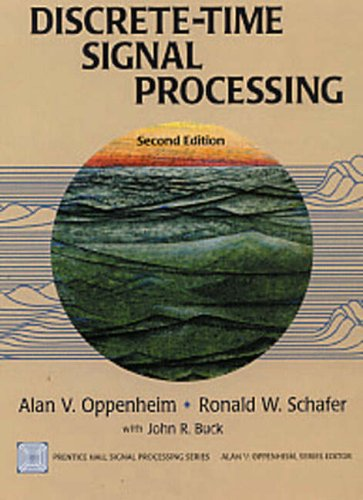
\includegraphics[width=.8\textwidth]{dtsp.jpg}\end{center}
    \column{.5\textwidth}
    {\bf\color{blue!50!black}ECES631} \\
    Fund. of Deterministic DSP \\
    \vspace{1em}
    
    {\bf\color{blue!50!black}Instructor} \\
    Dr. Gail Rosen ({\color{blue}\url{gailr@ece.drexel.edu}}) \\
    \vspace{1em}
    
    {\bf\color{blue!50!black}Office Hours} \\
    By appointment. \\
    \vspace{1em}

    
    {\bf\color{blue!50!black}Text} \\
    Oppenheim, Schafer \& Buck, ``Discrete-Time Signal Processing,'' 3rd Ed.
    \vspace{1em}
    
    {\bf\color{blue!50!black}Other Stuff}
    \begin{itemize}
      \item DSP is a {\em prerequisite}!
      \item Course materials are available on BBLearn.  
    \end{itemize}
    \vspace{1em}
  \end{columns}
\end{frame}



%--------------------------------------------------------------------------------------------
\begin{frame}\frametitle{What is DSP?}\small
  \begin{center}
    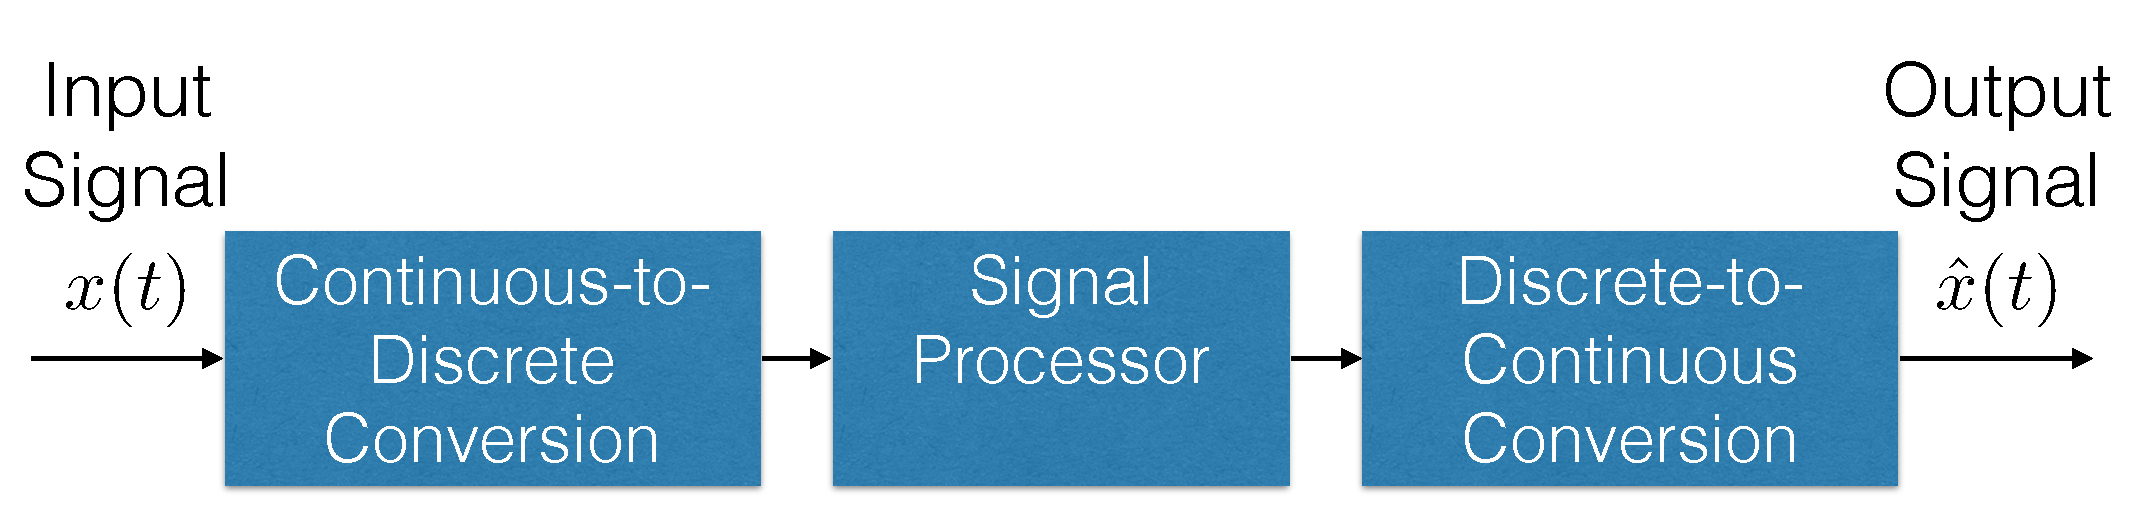
\includegraphics[width=.9\textwidth]{dsp_flow.pdf}
  \end{center}
  \begin{exampleblock}{\small Digital Signal Processing}
  \begin{itemize}
    \item {\bf\color{green!50!black}Digital} 
      \begin{itemize}
        \item Method to represent a quantity, a phenomenon or an event
        \item Why Digital?
      \end{itemize}
    \item {\bf\color{green!50!black}Signal}
      \begin{itemize}
        \item What is a signal?
        \item What are we interested in?
      \end{itemize}
    \item {\bf\color{green!50!black}Processing}
      \begin{itemize}
        \item What kind of processing do we need to perform?
        \item What special effects do we need to look out for?
      \end{itemize}
  \end{itemize}
  \end{exampleblock}
\end{frame}


%--------------------------------------------------------------------------------------------
\begin{frame}\frametitle{What is DSP?}\small
  \begin{center}
    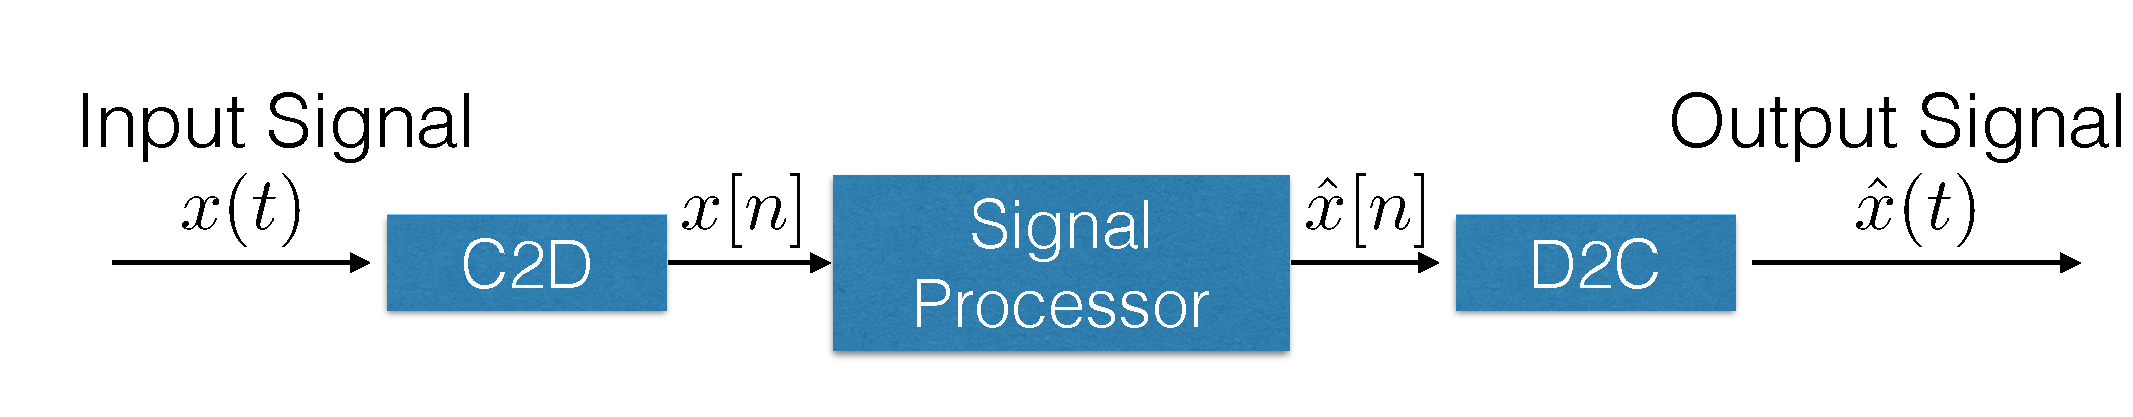
\includegraphics[width=.9\textwidth]{dsp_flow_sampled.pdf}
  \end{center}
  \begin{block}{\small Digital Signal Processing}
  \begin{itemize}
    \item What is a digital signal? Its just a sequence of numbers that can be represented as 
      \begin{align}
         x = \{x[n]\}, \hspace{3em} -\infty < n <  \infty \nonumber
      \end{align}
    \item $x[n]$ is sampled from an analog signal
      \begin{align}
         x[n] = x(nT_s) \hspace{3em} -\infty < n <  \infty \nonumber
      \end{align}
      where $T_s$ is the sampling period, which is the reciprocal of the sampling rate ($f_s$). 
  \end{itemize}
  \end{block}
\end{frame}


%--------------------------------------------------------------------------------------------
\begin{frame}\frametitle{Common sequences and operations}\small
  {\bf\color{blue!50!black}Unit and Impulse Sequences} \\
  The discrete unit step ($u[n]$), and impulse sequences $\delta[n]$ are among the most commonly utilized sequences in DSP. Why? 
  \begin{align}
     \delta[n] = \left\{ 
         \begin{array}{l l}
           1 & \textrm{if } n=0 \\
           0 & \textrm{otherwise}
         \end{array}
       \right.
     \hspace{3em}
     u[n] = \left\{ 
         \begin{array}{l l}
           1 & \textrm{if } n \geq 0 \\
           0 & \textrm{otherwise}
         \end{array}
       \right. = \sum_{k=-\infty}^{\infty} \delta[n]
     \nonumber
  \end{align}
  
  \uncover<2->{
  {\bf\color{blue!50!black}Exponential Sequences} \\
  The exponential sequences is important for representing and analyzing linear time-invariant discrete-time systems
  \begin{align}
    x[n] = A \alpha^n \nonumber
  \end{align}
  where if $A,\alpha \in \Rbb$ then $x[n] \in \Rbb$.\\
  \vspace{1em} 
  }
  
  \uncover<3->{
  {\bf\color{blue!50!black}Euler's Identities} \\
  Never forget!
  \begin{align}
    \cos(\omega n) = \frac{\e^{j\omega n} + \e^{-j\omega n}}{2}, \hspace{1em}
    \sin(\omega n) = \frac{\e^{j\omega n} - \e^{-j\omega n}}{j2} \nonumber \\
    \e^{j\omega n} = \cos(\omega n) + j \sin(\omega n), \hspace{1em}
    \e^{-j\omega n} = \cos(\omega n) - j \sin(\omega n)
    \nonumber
  \end{align}
  }
\end{frame}

%--------------------------------------------------------------------------------------------
\begin{frame}\frametitle{What do they look like?}\small
  \begin{center}
    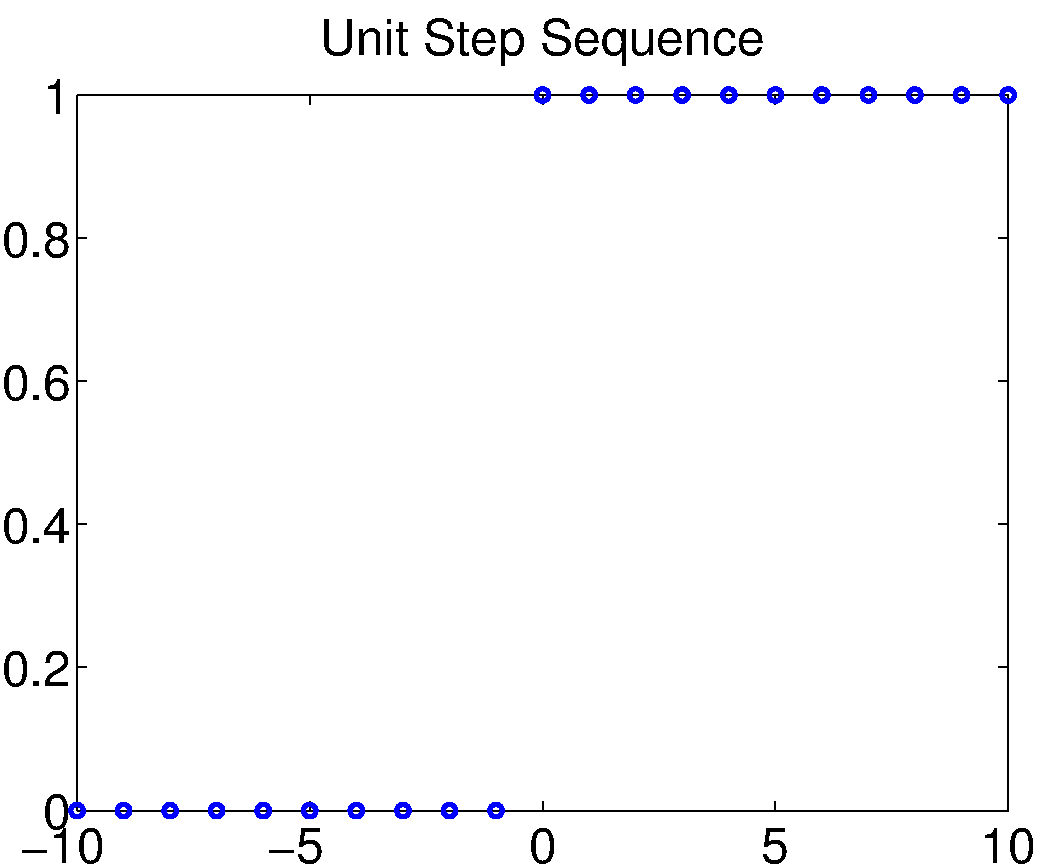
\includegraphics[width=.35\textwidth]{step_fcn.pdf} \hspace{1em}
    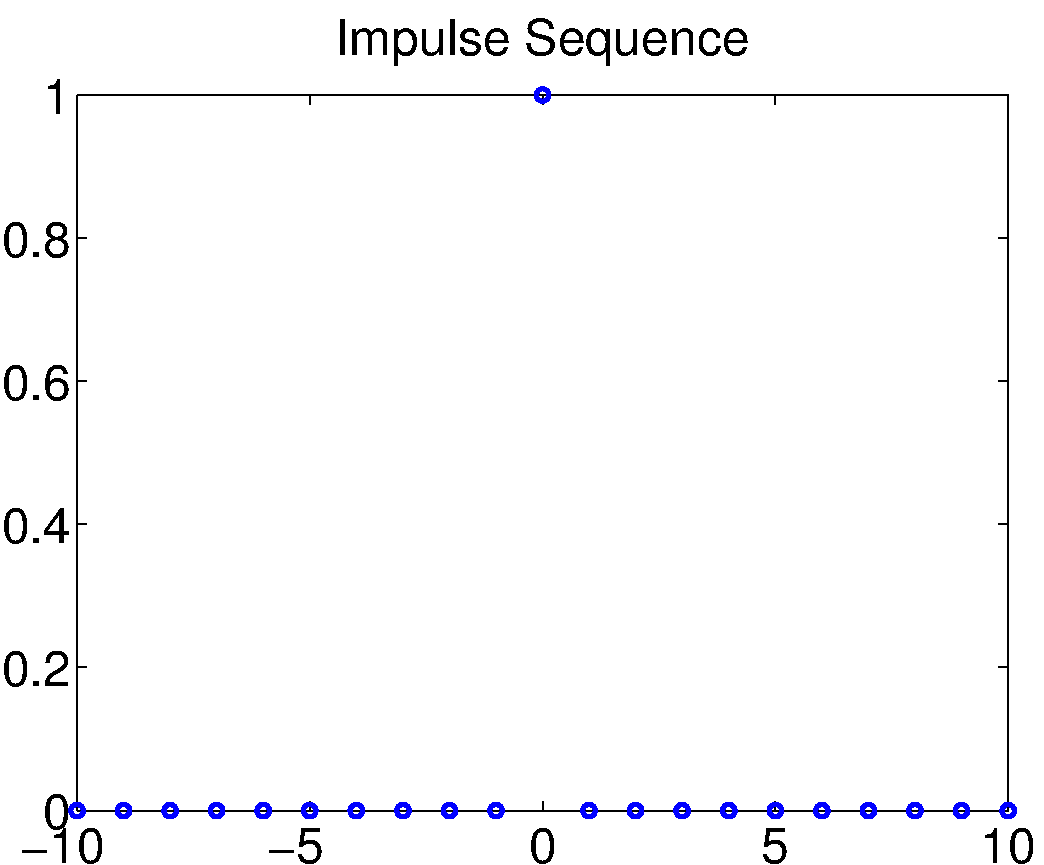
\includegraphics[width=.35\textwidth]{impulse_fcn.pdf}  \\
    \vspace{1em}
    
    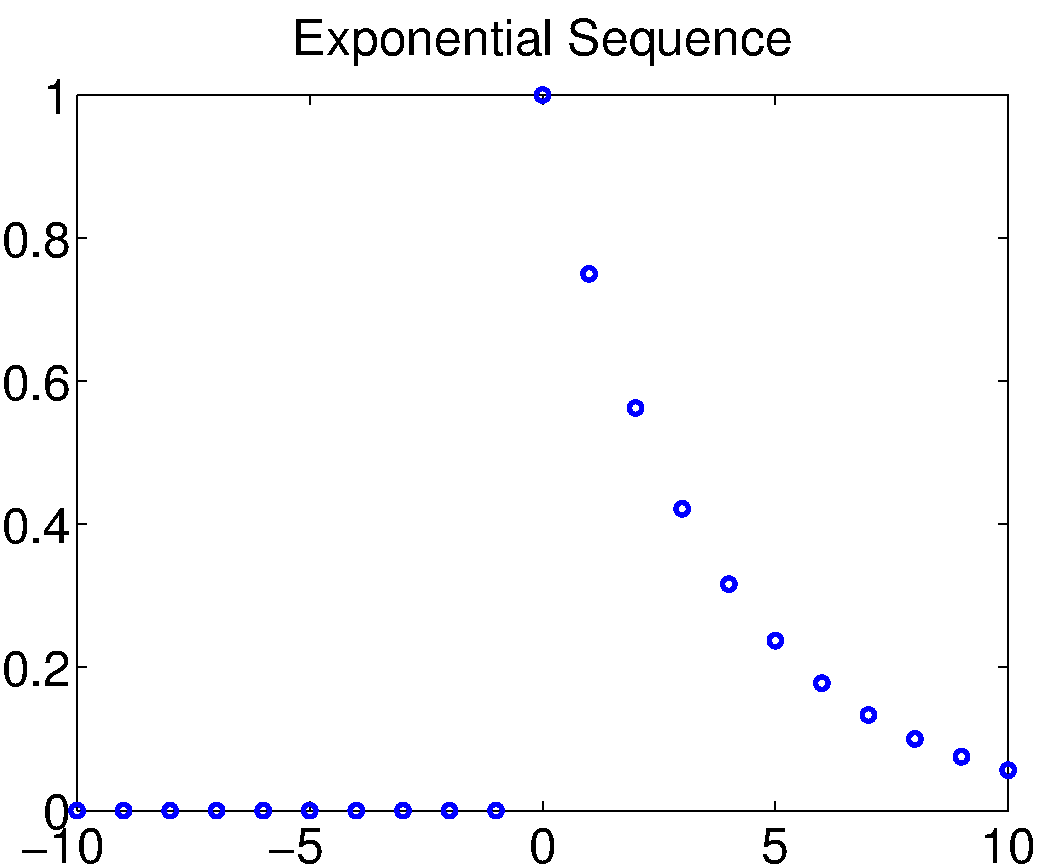
\includegraphics[width=.35\textwidth]{exp_fcn.pdf} \hspace{1em}
    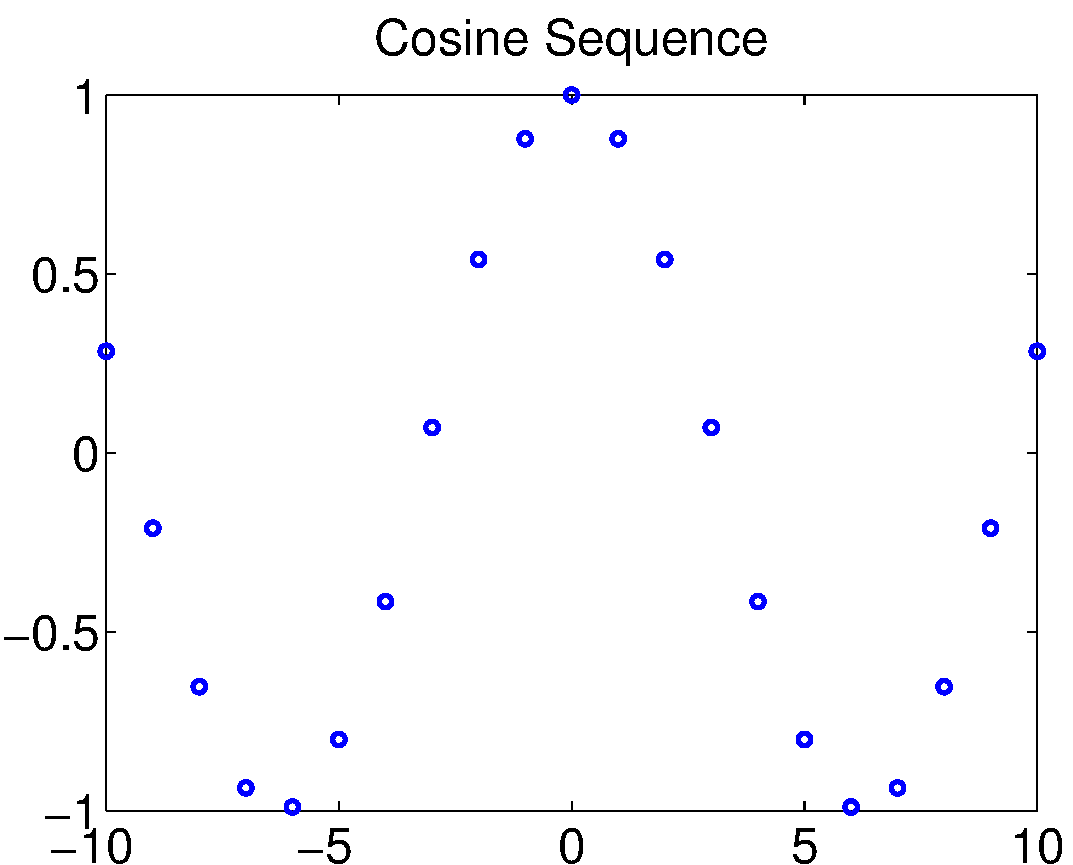
\includegraphics[width=.35\textwidth]{cos_fcn.pdf}
  \end{center}
\end{frame}


%--------------------------------------------------------------------------------------------
\begin{frame}\frametitle{Linear Systems}\small
  \begin{block}{What is a linear system?}
    A class {\em of linear systems} is defined by the property of superposition. Let $T$ be an operation, and $y_1[n]$ and $y_2[n]$ be the system responses of a system when $x_1[n]$ and $x_2[n]$ are the inputs, respectively. Then the system is linear if, and only if: 
    \begin{align}
      T\{x_1[n] + x_2[n]\} = T\{x_1[n]\} + T\{x_2[n]\} = y_1[n] + y_2[n]  \hspace{1em} \textrm{(additivity)}
      \nonumber
    \end{align}
    and 
    \begin{align}
      T\{ \alpha x[n]\} = \alpha T\{  x[n]\} = \alpha y[n] \hspace{1em} \textrm{(homogenity)}
      \nonumber
    \end{align}
    where $\alpha$ is an arbitrary constant. 
  \end{block}
  
  \uncover<2->{
  \begin{exampleblock}{Questions}
    Is an accumulator system given by  
    \begin{align}
      y[n] = \sum_{k=-\infty}^{n} x[k]
      \nonumber
    \end{align}
    a linear system?
  \end{exampleblock}
  }
\end{frame}

%--------------------------------------------------------------------------------------------
\begin{frame}\frametitle{Time-Invariant Systems}\small
  \begin{block}{What is time-invariance?}
    A system is said to be time-invariant if a delay on the input sequence results in an equal delay of the output sequence. That is, if $\hat{x}[n] = x[n-n_0]$ then $\hat{y}[n] = y[n-n_0]$. 
  \end{block}
  
  \uncover<2->{
  \begin{exampleblock}{The Accumulator as a Time-Invariant System}
    Define $x_i[n] = x[n-n_0]$ and let
    \begin{align}
    y[n - n_0] = \sum_{k=-\infty}^{n-n_0}x[k] \nonumber
    \end{align}
    Next, we have 
    \begin{align}
    y_1[n] = \sum_{k=-\infty}^{n}x_1[k] = \sum_{k=-\infty}^{n}x[k-n_0]\nonumber
    \end{align}
    Substituting the change of variables for $k_1=k-n_0$ into the sum gives
    \begin{align}
      y_1[n] = \sum_{k_1=-\infty}^{n-n_0}x[k_1] = y[n-n_0] 
      \nonumber
    \end{align}
  \end{exampleblock}
  }
\end{frame}


%--------------------------------------------------------------------------------------------
\begin{frame}\frametitle{Other Important Stuff}\small
  {\bf\color{blue!50!black}Causality} \\
  A system is casual if, for every choice of $n_0$, the output sequence value at the index $n=n_0$ depends only of the input sequence values for $n \leq n_0$. Is $y[n] = x[n+1] - x[n]$ causal? How about $y[n] = \log(x[|n| - n_0])$?\\
  \vspace{1em}
  
  {\bf\color{blue!50!black}Stability} \\
  A system is bounded-input bounded-output (BIBO) stable if and only if  every bounded input sequence results in a bounded output sequence. 
  \vspace{1em}
  
  {\bf\color{blue!50!black}Everything else} \\
  Seriously, read Chapter 2 of the text book!
\end{frame}


%--------------------------------------------------------------------------------------------
\begin{frame}\frametitle{Linear Time-Invariant Systems}\small
  \begin{block}{What are they?}
    \begin{itemize}
      \item As the name states, these systems are linear and time-invariant. They are one of the most important components to the field of digital signal processing. 
      \item An LTI system can be completely characterized by its impulse response. That is, $x[n] = \delta[n]$.
    \end{itemize}
  \end{block}
  
  \begin{exampleblock}{Convolution}
    \begin{itemize}
      \item The convolution of two sequences $x$ and $h$ is defined by:
        \begin{align}
          y[n] = \sum_{k=-\infty}^{\infty} x[k] h[n-k]  = x[n] \star h[n] \nonumber
        \end{align}
      \item The importance of the equation shown above cannot be overstated enough 
    \end{itemize}
  \end{exampleblock}
\end{frame}


%--------------------------------------------------------------------------------------------
\begin{frame}\frametitle{Convolution Example}\small
  \begin{center}
    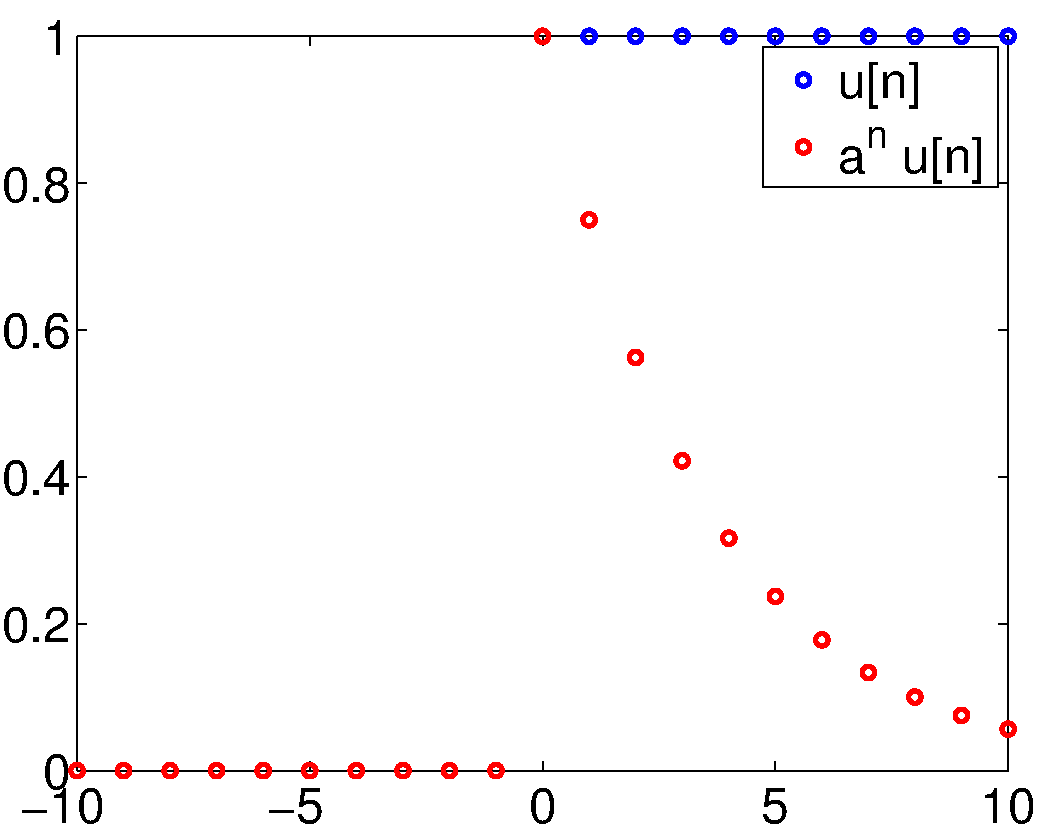
\includegraphics[width=.45\textwidth]{conv_00.pdf} \hspace{2em}
    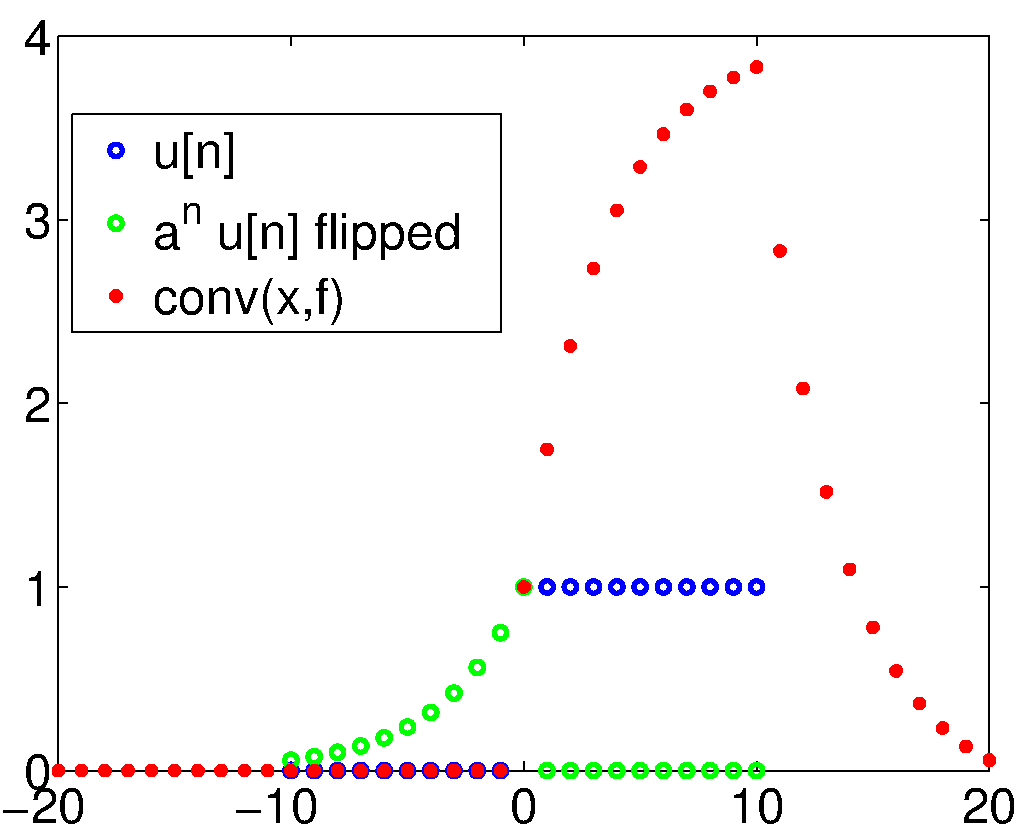
\includegraphics[width=.45\textwidth]{conv_01.pdf}
  \end{center}
\end{frame}

%--------------------------------------------------------------------------------------------
\begin{frame}\frametitle{Convolution Example}\small
  \begin{center}
    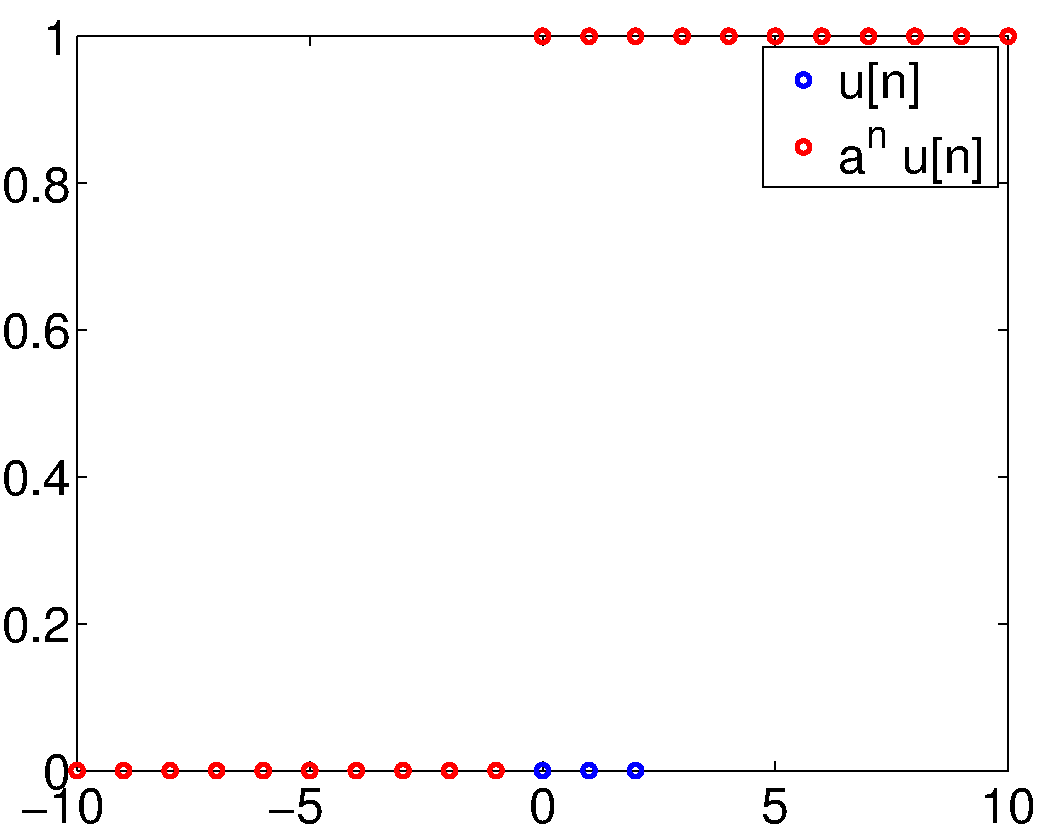
\includegraphics[width=.45\textwidth]{conv_02.pdf} \hspace{2em}
    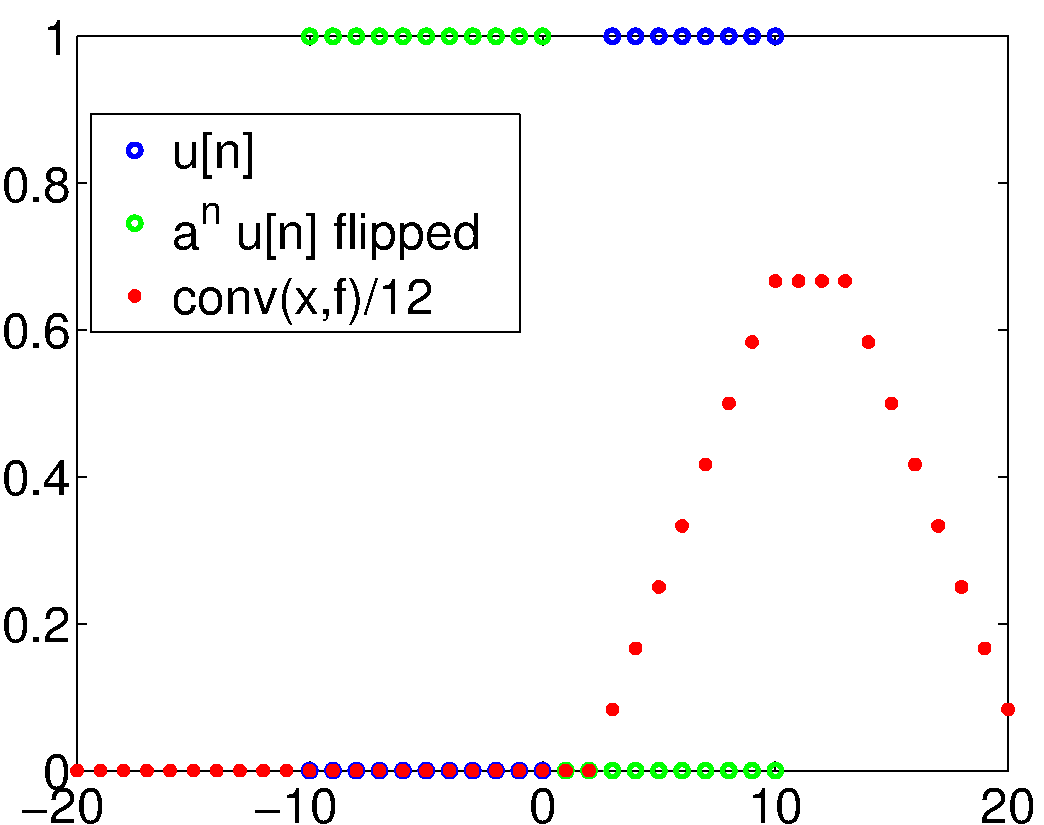
\includegraphics[width=.45\textwidth]{conv_03.pdf}
  \end{center}
\end{frame}

%--------------------------------------------------------------------------------------------
\begin{frame}\frametitle{Properties of LTI Systems}\small

  \begin{exampleblock}{Some Properties}
  \begin{itemize}
    \item An LTI system can be completely characterized by its impulse response.  
    \item Convolution is commutative, that is, $x[n] \star h[n] = h[n] \star x[n]$
      \begin{align}
        y[n] = \sum_{m=\infty}^{-\infty}{x[n-m]h[m]} = \sum_{m=-\infty}^{\infty}{h[m]x[n-m]} = h[n] \star x[n]
        \nonumber
      \end{align}
    \item For an LTI system with $h[n] = h_1[n] + h_2[n]$, we have
      \begin{align}
        x[n] \star \left( h_1[n] + h_2[n] \right) = h_1[n] \star x[n] + h_2[n] \star x[n]
        \nonumber
      \end{align}
  \end{itemize}
  \end{exampleblock}
\end{frame}





%--------------------------------------------------------------------------------------------
\begin{frame}\frametitle{Equivalence of LTI Systems}\small
  \begin{center}
    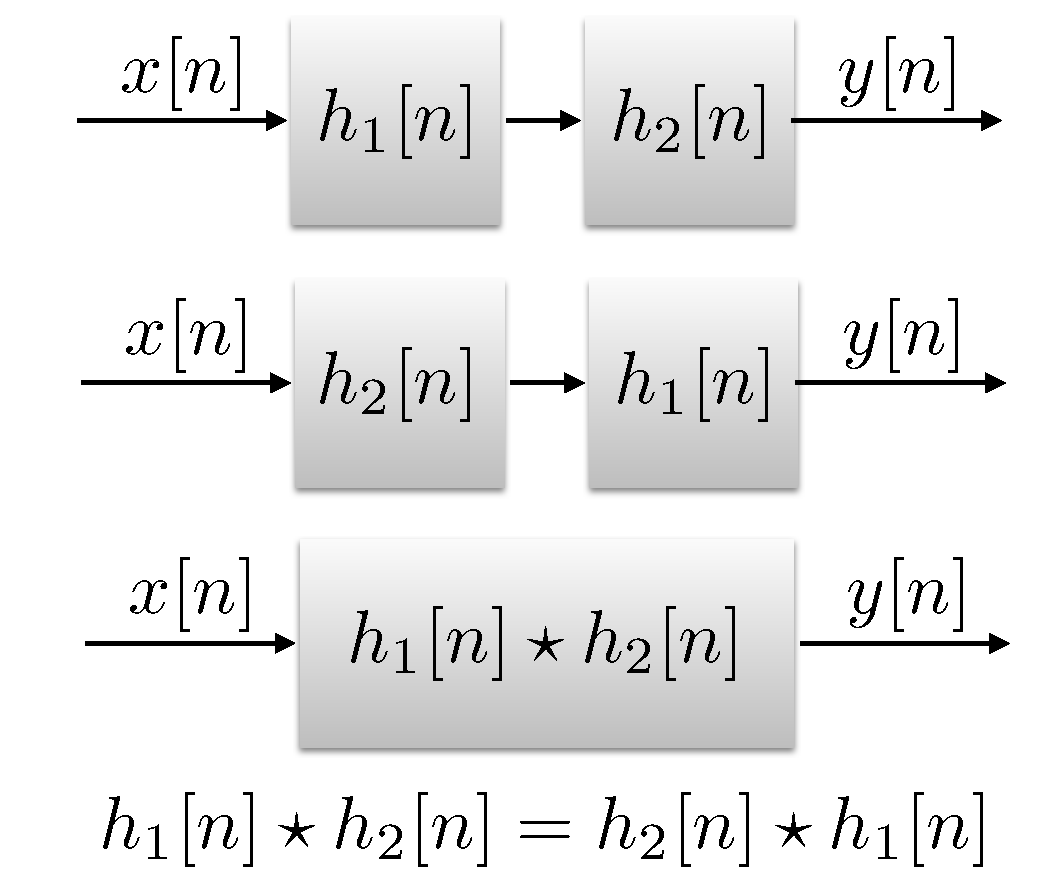
\includegraphics[height=.45\textheight]{lti_sys_00.pdf} \hspace{2em}
    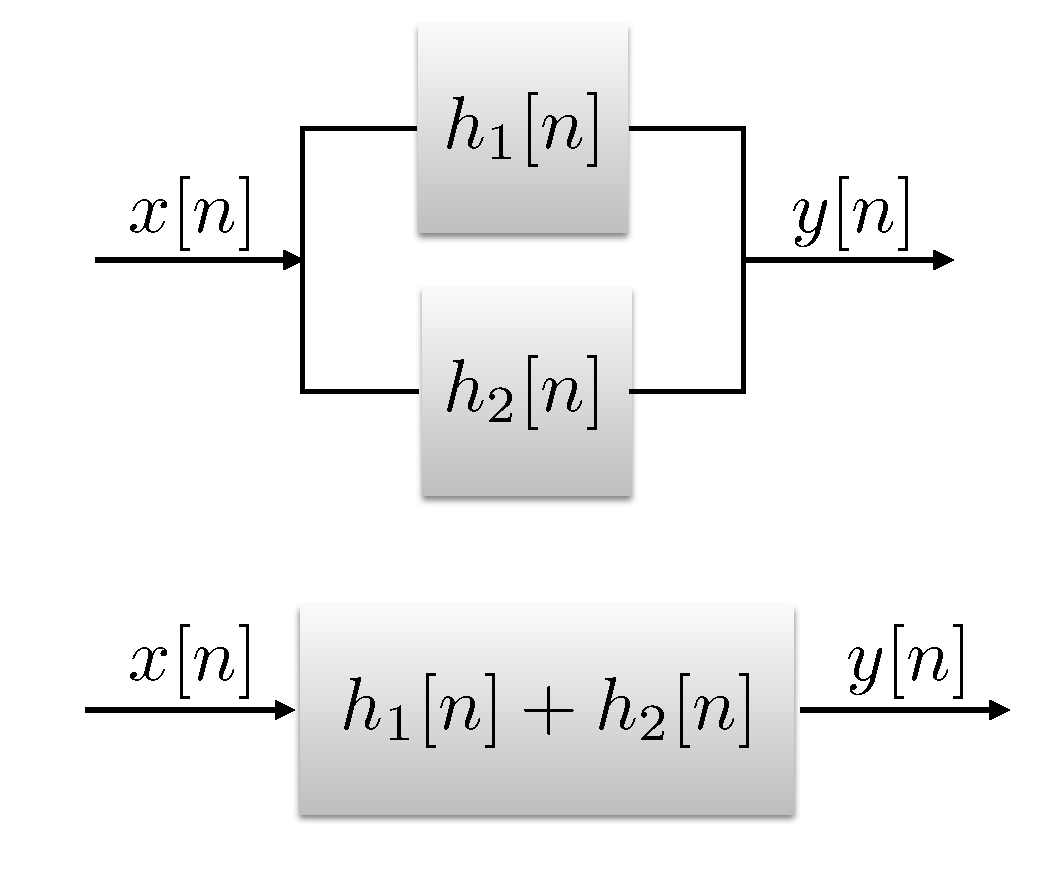
\includegraphics[height=.45\textheight]{lti_sys_01.pdf}
  \end{center}
\end{frame}



%--------------------------------------------------------------------------------------------
\begin{frame}\frametitle{LTI Examples: Moving Average}\small
  \begin{exampleblock}{}
  \begin{align}
    y[n] = \frac{1}{L} \sum_{k=0}^{L-1}x[n-k]
    \nonumber
  \end{align}
  \end{exampleblock}
  \uncover<2->{
  \noindent{\bf\color{blue!50!black}Linear?: }\uncover<3->{ Yes}\\
  \begin{align}
     \frac{1}{L} \sum_{k=0}^{L-1}(a x_1[n-k] + b x_2[n-k]) = a\left(\frac{1}{L} \sum_{k=0}^{L-1}x[n-k]\right) + b\left(\frac{1}{L} \sum_{k=0}^{L-1}x[n-k] \right)
    \nonumber
  \end{align}
  }
  \uncover<4->{
  \noindent{\bf\color{blue!50!black}Time-Invariant?:} \uncover<5->{Yes}\\
  \begin{align}
    \frac{1}{L} \sum_{k=0}^{L-1}x[n-k-n_0] = \frac{1}{L} \sum_{k=0}^{L-1}x[(n-n_0)-k] = y[n-n_0]
    \nonumber
  \end{align}
  }
  \uncover<6->{
  \noindent{\bf\color{blue!50!black}Casual?:} \uncover<7->{Yes}\\
  \begin{align}
    y[n] = \frac{1}{L}\left( x[n] + x[n-1] +\ldots + x[n-L+1] \right)
    \nonumber
  \end{align}
  }
  \uncover<8->{
  \noindent{\bf\color{blue!50!black}BIBO?:} \uncover<9->{Yes}\\
  \begin{align}
    |y[n]| = \left|\frac{1}{L} \sum_{k=0}^{L-1}x[n-k]\right| \leq \frac{1}{K} \sum_{k=0}^{L-1}|x[n-k]| \leq B_x
    \nonumber
  \end{align}
  }
\end{frame}


%--------------------------------------------------------------------------------------------
\begin{frame}\frametitle{LTI Examples: Downsampler}\small
  \begin{exampleblock}{}
  \begin{align}
    y[n] = x[Mn]
    \nonumber
  \end{align}
  \end{exampleblock}
  \uncover<2->{
  \noindent{\bf\color{blue!50!black}Linear?: } \uncover<3->{Yes}\\
  \begin{align}
     a x_1[Mn] + b x_2[Mn] = a y_1[n] + b y_2[n]
    \nonumber
  \end{align}
  }
  \uncover<4->{
  \noindent{\bf\color{blue!50!black}Time-Invariant?:} \uncover<5->{No}\\
  \begin{align}
    y_1[n] = x_1[Mn] = x[Mn - n_0] \neq y[n-n_0] = x[M(n-n_0)]
    \nonumber
  \end{align}
  }
  \uncover<6->{
  \noindent{\bf\color{blue!50!black}Casual?:} \uncover<7->{No}\\
  \begin{align}
    y[-1] = x[M],\textrm{but }y[1] = x[M] 
    \nonumber
  \end{align}
  }
  \uncover<8->{
  \noindent{\bf\color{blue!50!black}BIBO?:} \uncover<9->{Yes}\\
  \begin{align}
    |y[n]| = |x[Mn]| \leq B_x
    \nonumber
  \end{align}
  }
\end{frame}

%--------------------------------------------------------------------------------------------
\begin{frame}\frametitle{LTI Systems}\small
  
  \begin{columns}
  \column{.45\textwidth}
  \begin{block}{Ideal Delay}
    \begin{align}
    h[n] = \delta[n-n_0]
    \nonumber
    \end{align}
  \end{block}
  \begin{exampleblock}{Moving Average}
    \begin{align}
    h[n] &= \frac{1}{M_1+M_2+1}\sum_{k=-M_1}^{M_2}\delta[n-k]
    \nonumber \\
    &=
      \left\{
        \begin{array}{l l}
          \frac{1}{M_1+M_2+1} & -M_1 \leq n \leq M_2 \\
          0 & \textrm{otherwise}
        \end{array}
      \right.
    \nonumber
    \end{align}
  \end{exampleblock}
  \begin{block}{Forward Difference}
    \begin{align}
    h[n] = \delta[n+1] - \delta[n]
    \nonumber
    \end{align}
  \end{block}

  \column{.45\textwidth}
  \begin{exampleblock}{Backward Difference}
    \begin{align}
    h[n] = \delta[n] - \delta[n-1]
    \nonumber
    \end{align}
  \end{exampleblock}
  \begin{block}{Accumulator}
    \begin{align}
    h[n] &= \sum_{k=-M_1}^{M_2}\delta[k]
    \nonumber \\
    &=
      \left\{
        \begin{array}{l l}
          1 & n \geq 0 \\
          0 & n < 0
        \end{array}
      \right. = u[n]
    \nonumber
    \end{align}
  \end{block}
  \begin{exampleblock}{$\star$Constant Coefficient Linear Difference$\star$}
    \begin{align}
    \sum_{k=0}^{M} a_k y[n-k] = \sum_{m=0}^{M} b_m x[n-m]
    \nonumber
    \end{align}
  \end{exampleblock}
  \end{columns}
\end{frame}



%--------------------------------------------------------------------------------------------
\begin{frame}\frametitle{Frequency Domain Representations of Discrete Signals}\small
  \begin{center}
    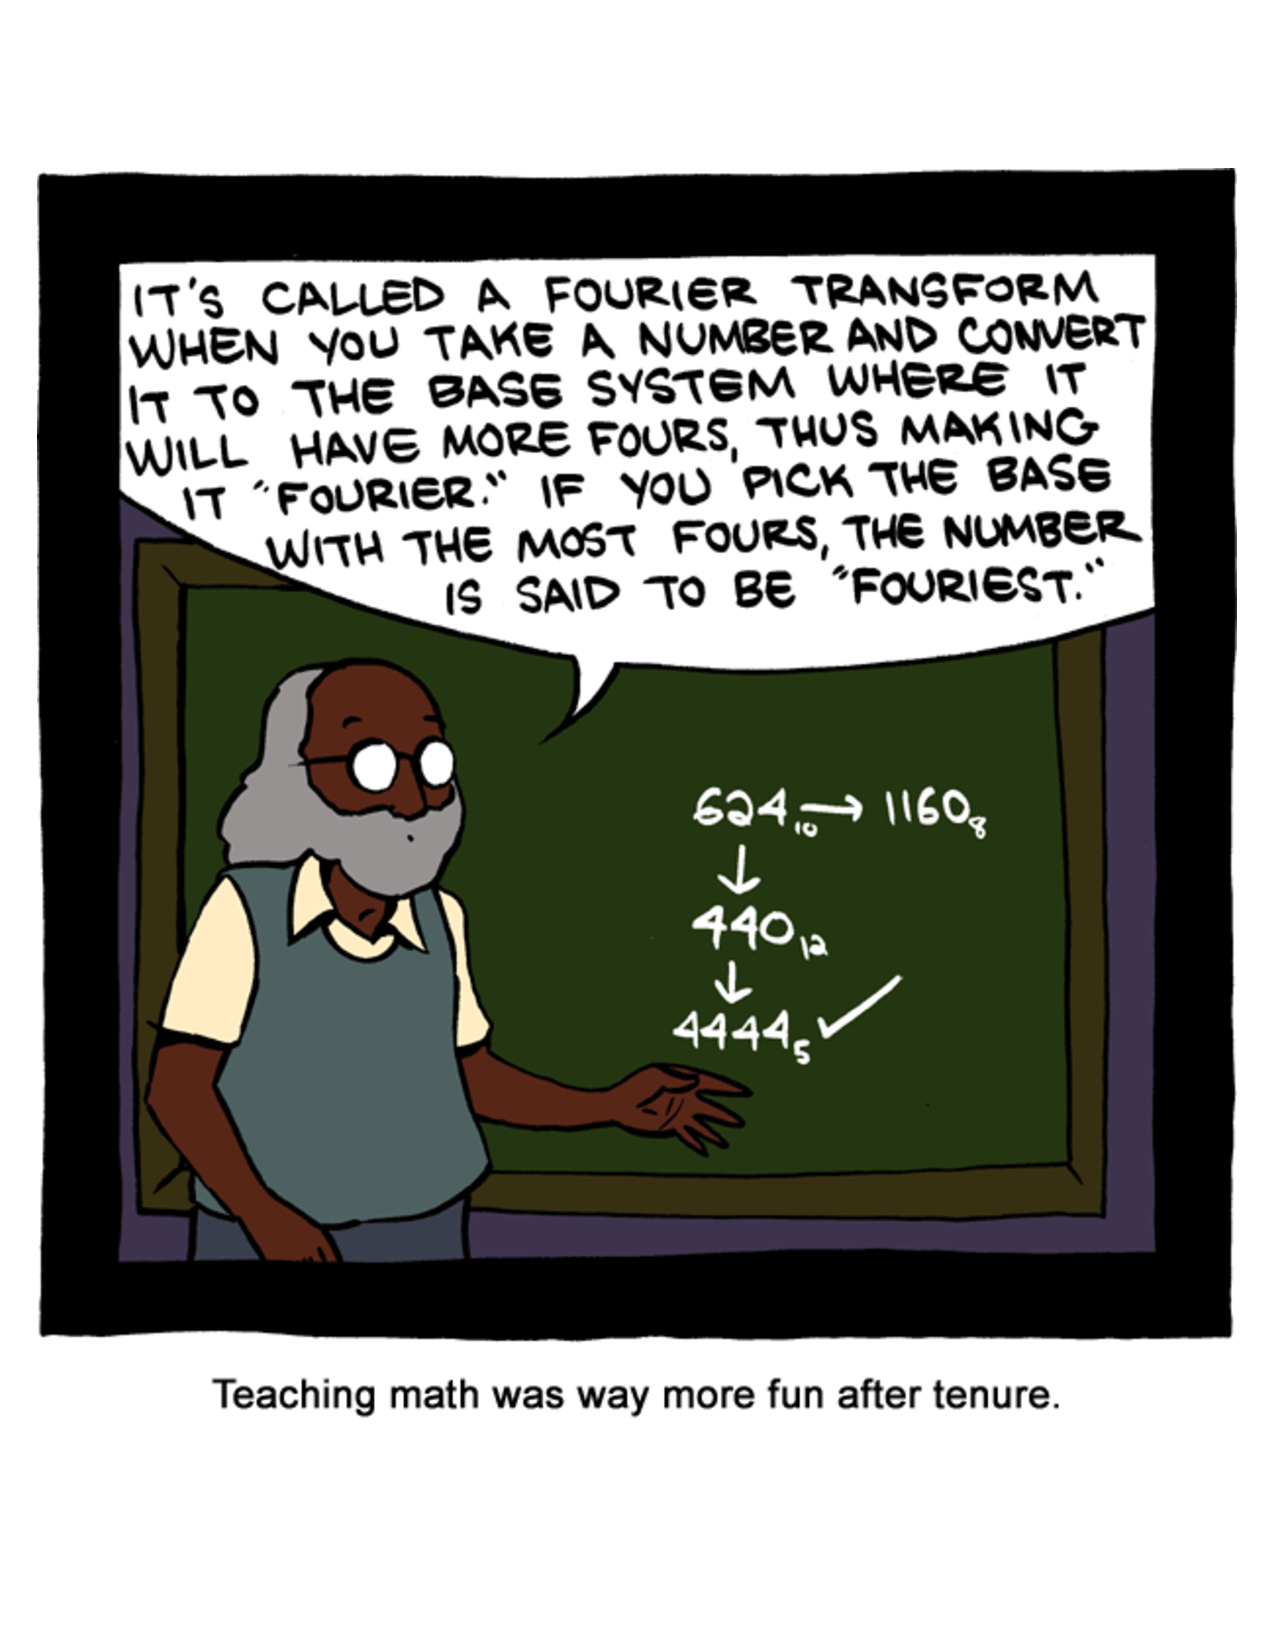
\includegraphics[height=\textheight]{fourier.pdf}
  \end{center}
\end{frame}

%--------------------------------------------------------------------------------------------
\begin{frame}\frametitle{Frequency Domain Representations of Discrete Signals}\small
  \begin{block}{LTI Systems}
    \begin{itemize}
      \item LTI systems can be written as a weighted sum of delayed impulse response coefficients. Until this point, we have only considered time domain representations of signals.   
      \item Recall a sinusoid can be written as a complex exponential functions, and as it turns out, complex exponential sequences are eigenfunctions of a LTI system. 
    \end{itemize}
  \end{block}
  
  \uncover<2->{
  \begin{exampleblock}{Eigenfunctions for LTI Systems}
    To demonstrate the eigenfunction property of LTI systems, let $x[n] = \e^{j\omega n}$, then 
    \begin{align}
      y[n] = \sum_{k=-\infty}^{\infty}h[n-k] \e^{-j\omega(n-k)} = \e^{j\omega} \left(\sum_{k=-\infty}^{\infty}h[n-k] \e^{-jk}\right) \nonumber
    \end{align}
    If $H(\e^{j\omega}) = \sum_{k=-\infty}^{\infty}{h[k]\e^{-j\omega k}}$, then 
    \begin{align}
      y[n]  = H(\e^{j\omega})\e^{j\omega n} \nonumber
    \end{align}
    Thus, $\e^{j\omega n}$ is an eigenfunction with a corresponding eigenvalue $H(\e^{j\omega})$. Furthermore, for convenience, we may write $H(\e^{j\omega})$ as $|H(\e^{j\omega})| \e^{j\angle H(\e^{j\omega})}$.
  \end{exampleblock}
  }
\end{frame}

%--------------------------------------------------------------------------------------------
\begin{frame}\frametitle{Frequency Domain Example}
   
   \begin{block}{Question}
   Find the frequency response of a moving averaging system  given by: 
   \begin{align}
     h[n] = \left\{
       \begin{array}{l l}
         \frac{1}{M_1+M_2+1} & -M_1 \leq n \leq M_2 \\
         0 & \textrm{otherwise}
       \end{array}
     \right. \nonumber
   \end{align}
   \end{block}
\end{frame}


%--------------------------------------------------------------------------------------------
\begin{frame}\frametitle{Frequency Domain Example}\small

  Therefore, the frequency response is given by 
  \begin{align}
    H(\e^{j\omega}) &= \frac{1}{M_1+M_2+1} \sum_{n=-M_1}^{M_2} \e^{-j\omega} \nonumber \\
    \uncover<2->{
    &=\frac{1}{M_1+M_2+1} \frac{\e^{j\omega M_1} - \e^{-j\omega (M_2 +1)}}{1 - \e^{-j\omega}} \nonumber }\\
    \uncover<3->{
    &=\frac{1}{M_1+M_2+1} \frac{\e^{j\omega (M_1+M_2+1)/2} - \e^{-j\omega (M_1+M_2+1)/2}}{1 - \e^{-j\omega}} \e^{-j\omega (M_2-M_1+1)/2}\nonumber }\\
    \uncover<4->{
    &=\frac{1}{M_1+M_2+1} \frac{\e^{j\omega (M_1+M_2+1)/2} - \e^{-j\omega (M_1+M_2+1)/2}}{ \e^{j\omega/2} -\e^{-j\omega/2} } \e^{-j\omega (M_2-M_1)/2}\nonumber }\\
    \uncover<5->{
    &=\frac{1}{M_1+M_2+1} \frac{ \sin\left( \omega (M_1+M_2+1)/2 \right) }{ \sin(\omega/2) } \e^{-j\omega (M_2-M_1)/2}\nonumber }
  \end{align}   
   
\end{frame}

%--------------------------------------------------------------------------------------------
\begin{frame}\frametitle{Frequency Domain Example}\small

  \begin{center}
     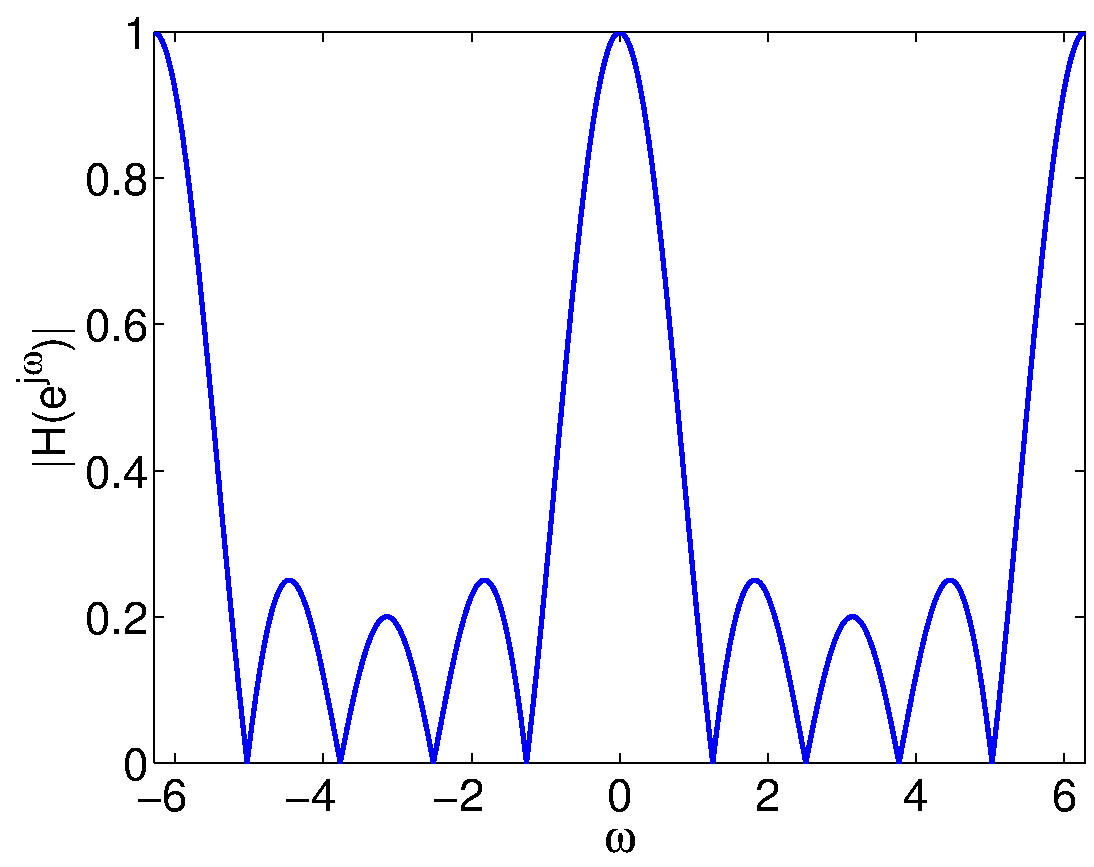
\includegraphics[width=.45\textwidth]{frmas_f.pdf}\hspace{1em}
     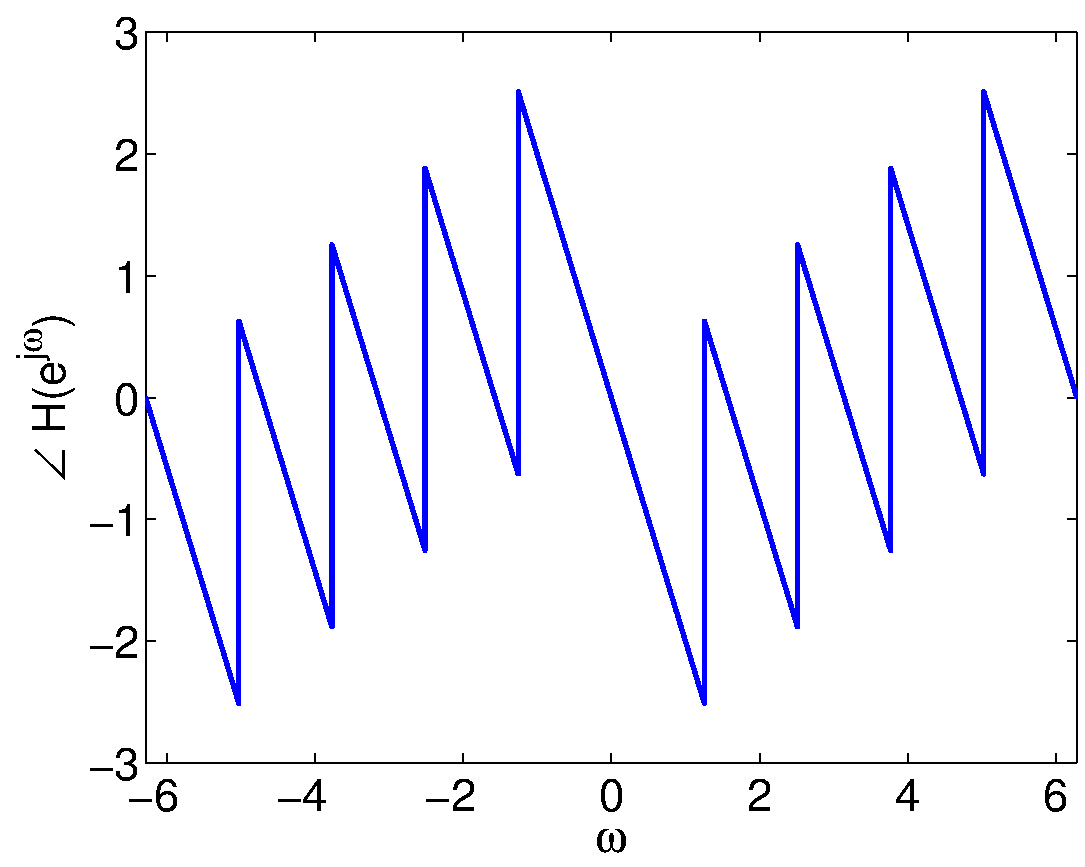
\includegraphics[width=.45\textwidth]{frmas_a.pdf}
  \end{center}
   
\end{frame}

%--------------------------------------------------------------------------------------------
\begin{frame}\frametitle{Historical Note: The  1889 World's Fair in Paris, France}\small
  \begin{center}
     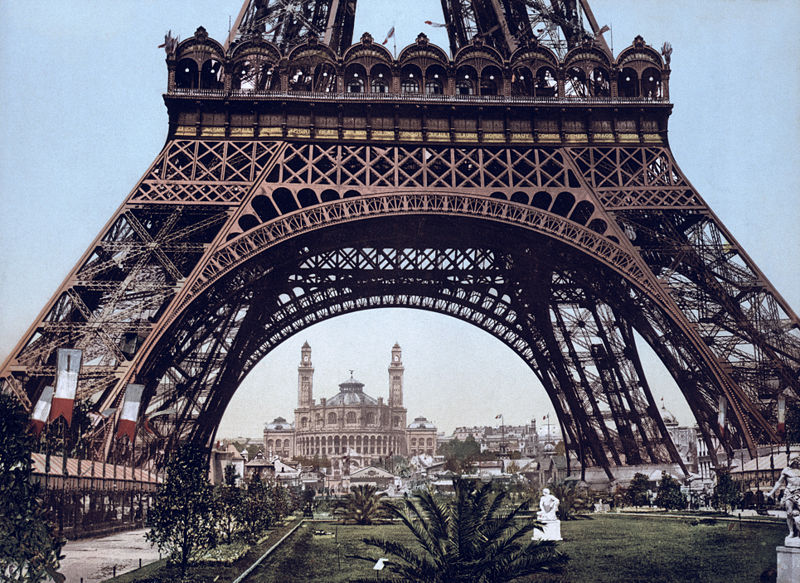
\includegraphics[width=.9\textwidth]{eiffel.jpg}\hspace{1em}
  \end{center}
\end{frame}

%--------------------------------------------------------------------------------------------
\begin{frame}\frametitle{And Who Made the List?}\small
  \begin{center}
     
\includegraphics[width=.9\textwidth]{F1.png}\hspace{1em} \\
     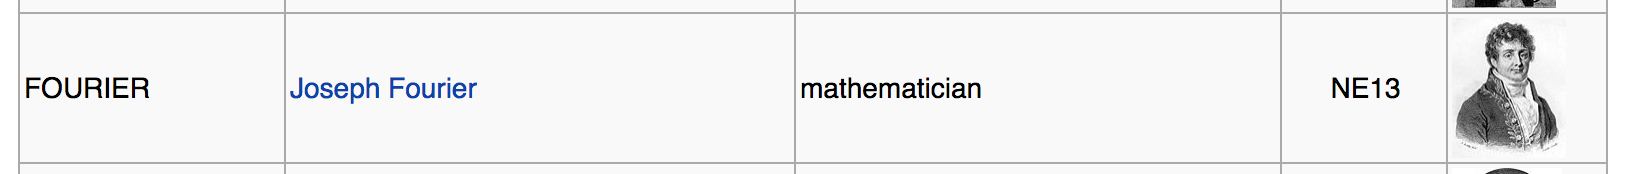
\includegraphics[width=.9\textwidth]{F2.png}\hspace{1em} \\
     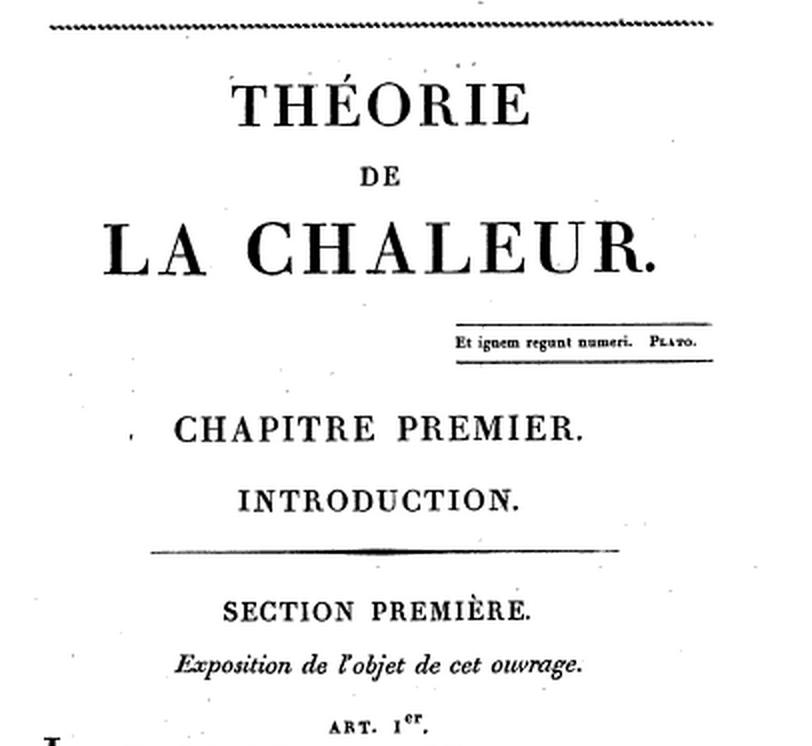
\includegraphics[height=.4\textheight]{f3.png}\hspace{1em} 
     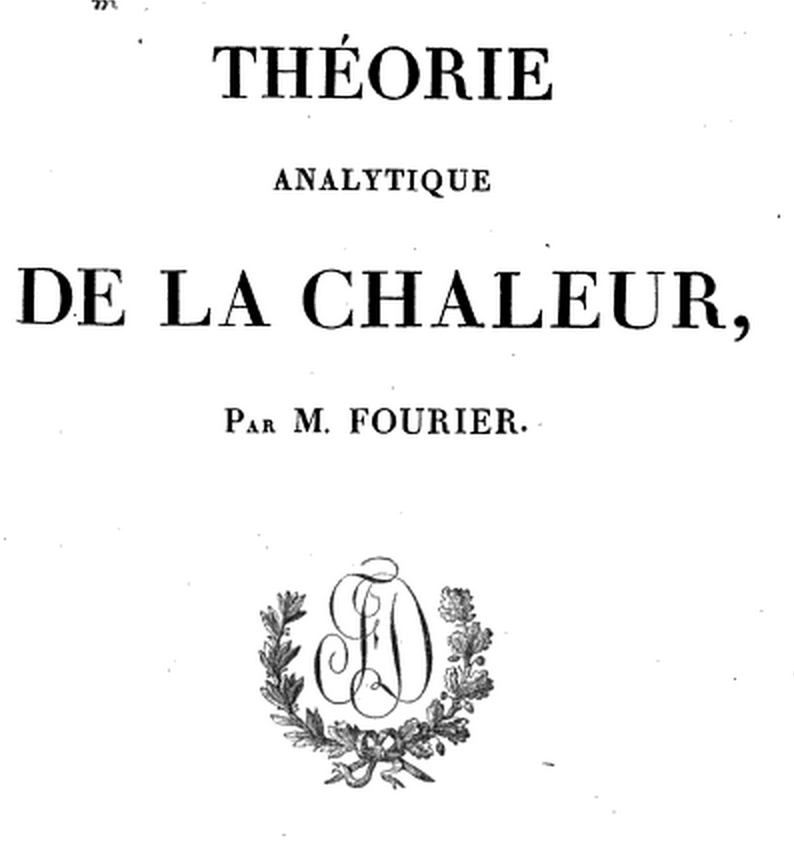
\includegraphics[height=.4\textheight]{f4.png}\hspace{1em} 
  \end{center}
\end{frame}


%--------------------------------------------------------------------------------------------
\begin{frame}\frametitle{The Discrete-Time Fourier Transform}
   
   \begin{block}{Discrete Fourier-Time Transform (Analysis)}
   The frequency spectrum for some signal $x[n]$ can be represented by: 
   \begin{align}
     X(\e^{j\omega}) = \sum_{n=-\infty}^{\infty} x[n] \e^{-j\omega n}
     \nonumber
   \end{align}
   \begin{itemize}
     \item For convenience, we write $\angle X(\e^{j\omega}) \in [\pm\pi]$. 
   \end{itemize}
   \end{block}
   
   \begin{exampleblock}{Inverse Discrete-Time Fourier Transform (Synthesis)}
   Any discrete sequence can be represented by: 
   \begin{align}
     x[n] = \frac{1}{2\pi} \int\limits_{-\pi}^{\pi} X(\e^{j\omega}) \e^{j\omega n} \d\omega
     \nonumber
   \end{align}
   \end{exampleblock}
\end{frame}



%--------------------------------------------------------------------------------------------
\begin{frame}\frametitle{Example}\small
   
   \begin{alertblock}{Absolute Summability for a Suddenly-Applied Exponential}
   Let $x[n] = a^n u[n]$. The Discrete-Time Fourier transform of this sequence is  
   \begin{align}
     X(\e^{j\omega}) &= \sum_{n=-\infty}^{\infty} x[n] \e^{-j\omega n}
     = \sum_{n=0}^{\infty} a^n \e^{-j\omega n}
     = \sum_{n=0}^{\infty} \left(a \e^{-j\omega}\right)^n
     \nonumber \\
     &= \frac{1}{1 - a \e^{-j\omega}} \nonumber
   \end{align}
   if $|a \e^{-j\omega}| < 1$ or $a < 1$. Clearly, the condition $a<1$ is the condition for the absolute summability of $x[n]$; i.e.,
   \begin{align}
      \sum_{n=0}^{\infty} |a|^n = \frac{1}{1-|a|} < \infty
     \nonumber
   \end{align} 
   again, only if $a < 1$. 
   \end{alertblock}
   
\end{frame}


%--------------------------------------------------------------------------------------------
\begin{frame}\frametitle{Example}\small
   
   \begin{exampleblock}{Low Pass Filter}
   Let us deterring the impulse response of an {\em ideal} low-pass filter. The frequency response is given by: 
   \begin{align}
     H_{\textrm{lp}}(\e^{j\omega}) = \left\{
       \begin{array}{l l}
         1 & |\omega| < \omega_c \\
         0 & \omega_c < |\omega| \leq \pi
       \end{array}
     \right.
     \nonumber
   \end{align}
   \uncover<2->{Then} 
   \begin{align}
     \uncover<2->{h_{\textrm{lp}}[n] &= \frac{1}{2\pi} \int\limits_{-\pi}^{\pi} H_{\textrm{lp}}(\e^{j\omega}) \e^{j\omega n} \d\omega}
     \uncover<3->{= \frac{1}{2\pi} \int\limits_{-\omega_c}^{\omega_c} \e^{j\omega n} \d\omega}\uncover<4->{ = \frac{1}{j 2\pi n} \left[ \e^{j\omega n} \right]_{\omega=-\omega_c}^{\omega=\omega_c}}
     \nonumber \\
     \uncover<5->{&= \frac{1}{j 2\pi n} \left( \e^{j\omega n} - \e^{-j\omega n} \right) = \frac{\sin(\omega_c n)}{\pi n}}
     \nonumber
   \end{align}
   \end{exampleblock}
   
   \uncover<6->{
   \begin{alertblock}{Notes}
   \begin{itemize}
     \item The impulse sequence $h_{\textrm{lp}}[n]$ is not zero for $n < 0$, and $h_{\textrm{lp}}[n]$ is not absolutely summable. 
     \item {\bf\color{red}Super Important Tip}: See Table 2.1 on page 56 of DTSP. 
   \end{itemize}
   \end{alertblock}
   }
\end{frame}

%--------------------------------------------------------------------------------------------
\begin{frame}\frametitle{Example of Gibbs Phenomenon}\small
  \begin{center}
    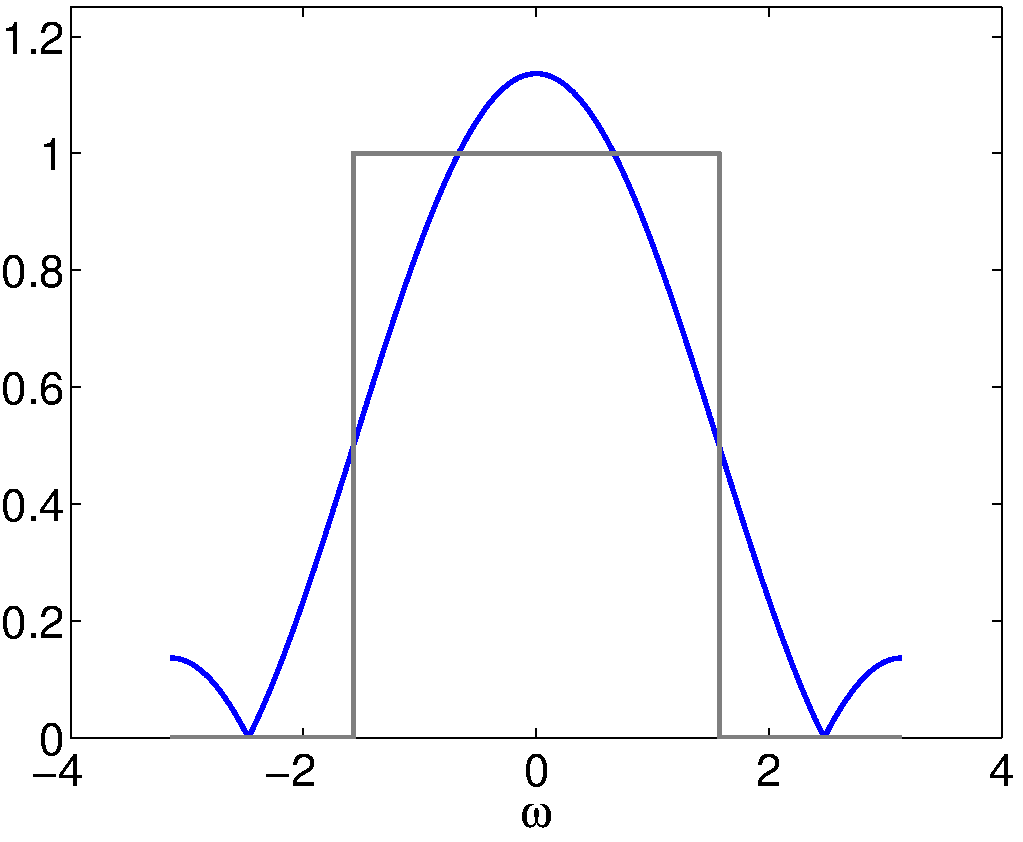
\includegraphics[width=.35\textwidth]{gibbs01.pdf} \hspace{1em}
    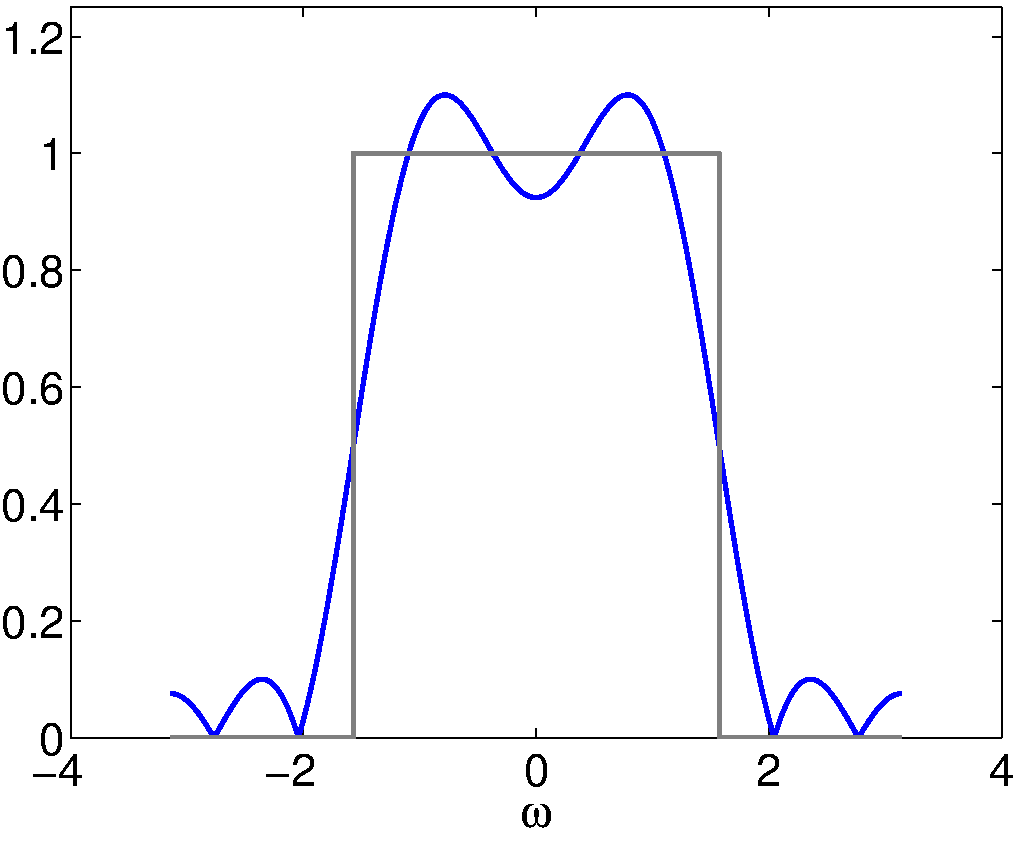
\includegraphics[width=.35\textwidth]{gibbs02.pdf}  \\
    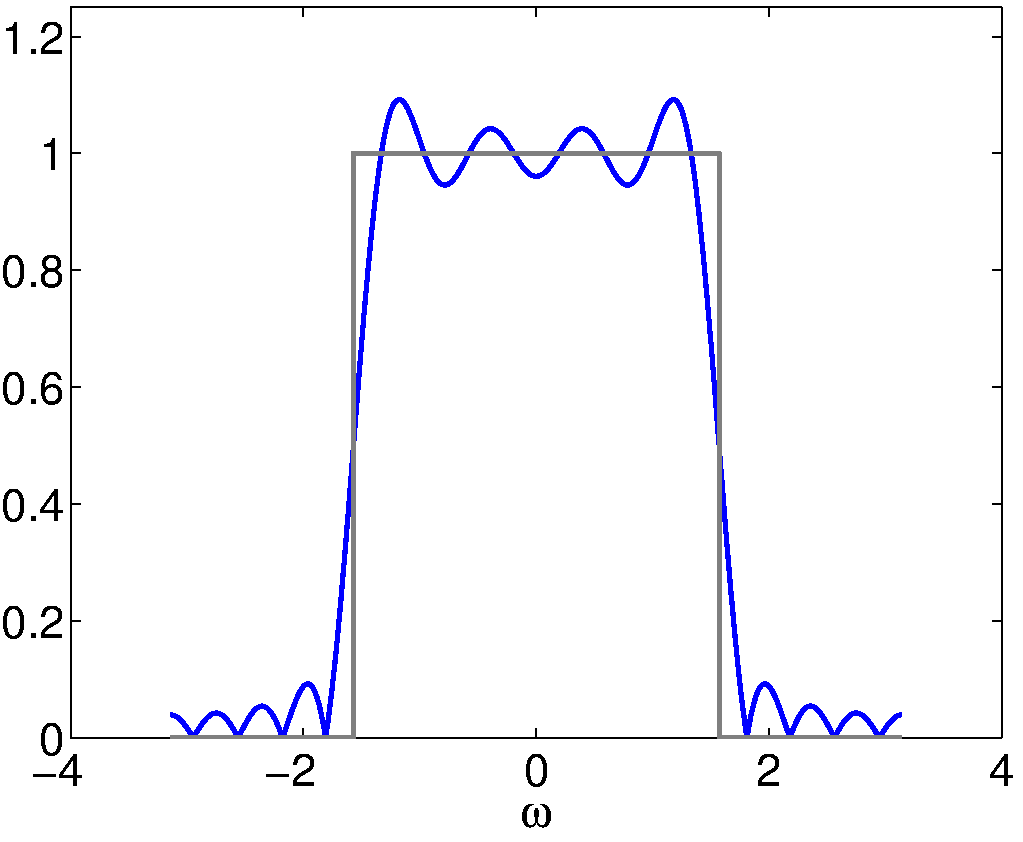
\includegraphics[width=.35\textwidth]{gibbs03.pdf} \hspace{1em}
    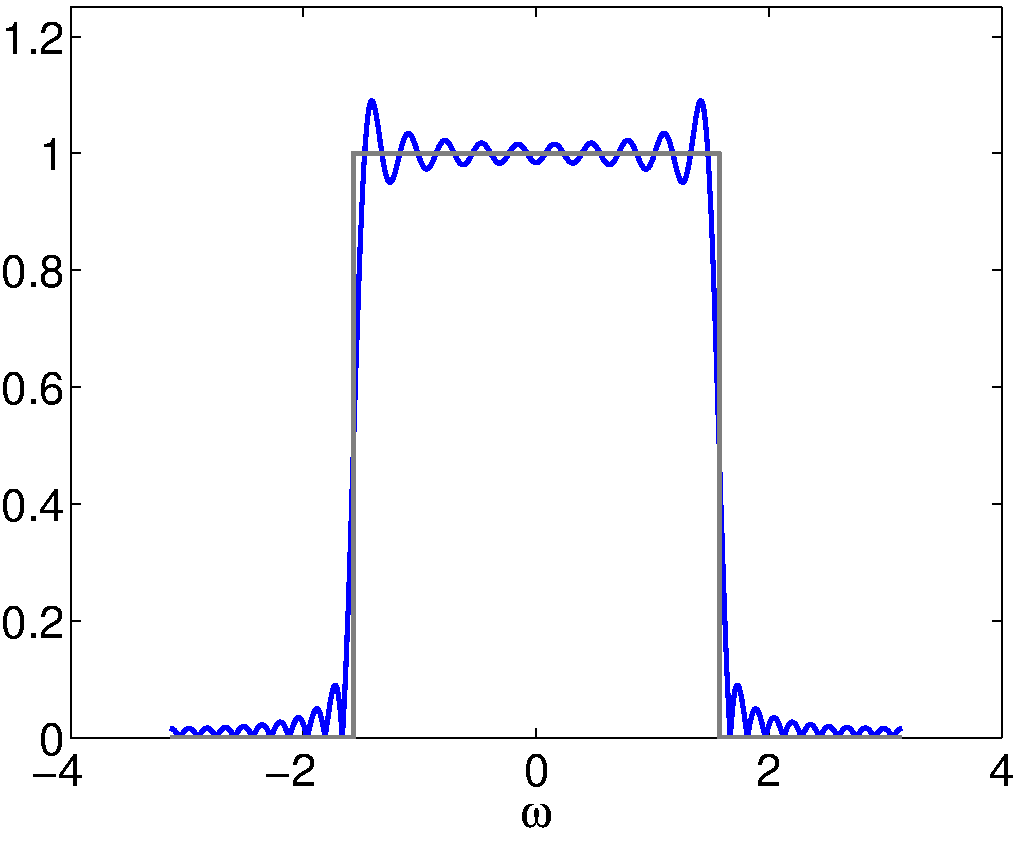
\includegraphics[width=.35\textwidth]{gibbs04.pdf}
  \end{center}
\end{frame}


%--------------------------------------------------------------------------------------------
\begin{frame}\frametitle{Parseval's Theorem}\small
  \begin{block}{\small General Idea}
    \begin{itemize} 
      \item Parseval's theorem provides a convenient way to compute the energy of a signal in the time-domain or frequency domain. In physics, this theorem is commonly referred to as the the Plancherel theorem. 
    \end{itemize}
  \end{block}
  
  \uncover<2->{
  \begin{exampleblock}{\small Derivation}
    \footnotesize
    \begin{align}
      \alert<8->{\frac{1}{2\pi} \int\limits_{-\pi}^{\pi} | X(\e^{j\omega}) |^2 \d\omega} 
         &= \frac{1}{2\pi} \int\limits_{-\pi}^{\pi}  X(\e^{j\omega}) X^*(\e^{j\omega})\d\omega 
          \uncover<3->{= \frac{1}{2\pi} \int\limits_{-\pi}^{\pi} \left( \sum_{n=-\infty}^{\infty} x[n] \e^{-j\omega n} \right) \left( \sum_{n'=-\infty}^{\infty} x^*[n'] \e^{j\omega n'} \right) \d\omega\nonumber} \\
         \uncover<4->{&= \frac{1}{2\pi} \int\limits_{-\pi}^{\pi}  \sum_{n=-\infty}^{\infty} x[n] \sum_{n'=-\infty}^{\infty} x^*[n'] \e^{j\omega (n' -n)} \d\omega \nonumber} \\
         \uncover<5->{&= \sum_{n=-\infty}^{\infty} x[n] \sum_{n'=-\infty}^{\infty} x^*[n']  \underbrace{\frac{1}{2\pi} \int\limits_{-\pi}^{\pi} \e^{j\omega (n' -n)}}_{ \left\{ \begin{tabular}{l l} $1$ & $n = n'$ \\ $0$ & \textrm{otherwise}  \end{tabular} \right. } \d\omega }
         \uncover<6->{= \sum_{n=-\infty}^{\infty} x[n]x^*[n] }
         \alert<8->{\uncover<7->{= \sum_{n=-\infty}^{\infty}| x[n]|^2 }}
         \nonumber
    \end{align}
  \end{exampleblock}
  }
\end{frame}

%--------------------------------------------------------------------------------------------
\begin{frame}\frametitle{Properties of the Discrete-Time Fourier Transform}\small
  \begin{block}{\small A Few other use properties ($x[n] \leftrightarrow X(\e^{j\omega})$)}
    \begin{itemize}
      \item If $y[n] = h[n] \star x[n]$ then $Y(\e^{j\omega}) = H(\e^{j\omega}) X(\e^{j\omega})$. This is the {\em Convolution Theorem}. 
      \item {\color{blue!50!black}Frequency Differentiation}%: If $x[n] \leftrightarrow X(\e^{j\omega})$
        \begin{align}
          n x[n] \leftrightarrow j \frac{\d X(\e^{j\omega})}{\d\omega}
          \nonumber
        \end{align}
      \item {\color{blue!50!black}Time Shifting}
        \begin{align}
          x[n-n_0] \leftrightarrow \e^{j\omega n_0} X(\e^{j\omega})
          \nonumber
        \end{align}
      \item {\color{blue!50!black}Frequency Shifting} 
        \begin{align}
          \e^{j\omega_0 n} x[n] \leftrightarrow  X\left(\e^{j(\omega - \omega_0)}\right)
          \nonumber
        \end{align}
    \end{itemize}
  \end{block}
\end{frame}


%--------------------------------------------------------------------------------------------
\begin{frame}\frametitle{Discrete-Time Fourier Transforms using Tables}\small
  Suppose that 
  \begin{align}
    X(\e^{j\omega}) = \frac{1}{\left(1 - a \e^{j\omega}\right)\left(1 - b \e^{j\omega}\right)} \nonumber
  \end{align}
  for $a \neq b$. \uncover<2->{Using the equation for the inverse discrete-time Fourier transform leads to an integral that is difficult to evaluate.} \uncover<3->{However, we can use partial fraction expansion to put $X(\e^{j\omega})$ in a form where we can use tables of transforms. 
  \begin{align}
    X(\e^{j\omega}) = \frac{\frac{a}{a-b}}{1 - a \e^{j\omega}} + \frac{\frac{b}{a-b}}{1 - b \e^{j\omega}} \nonumber
  \end{align}
  } \uncover<4->{After of examining tables with discrete-time Fourier transform leads to
  \begin{align}
    x[n] = \left( \frac{a}{a-b} \right) a^n u[n] - \left( \frac{b}{a-b} \right) b^n u[n]
    \nonumber
  \end{align}
  }
\end{frame}


%--------------------------------------------------------------------------------------------
\begin{frame}\frametitle{Discrete-Time Fourier Transforms using Tables}\small
  Suppose that 
  \begin{align}
    X(\e^{j\omega}) = \frac{1}{\left(1 - a \e^{j\omega}\right)\left(1 - b \e^{j\omega}\right)} \nonumber
  \end{align}
  for $a \neq b$. Using the equation for the inverse discrete-time Fourier transform leads to an integral that is difficult to evaluate. However, we can use partial fraction expansion to put $X(\e^{j\omega})$ in a form where we can use tables of transforms. 
  \begin{align}
    X(\e^{j\omega}) = \frac{\frac{a}{a-b}}{1 - a \e^{j\omega}} + \frac{\frac{b}{a-b}}{1 - b \e^{j\omega}} \nonumber
  \end{align}
  After of examining tables with discrete-time Fourier transform leads to
  \begin{align}
    x[n] = \left( \frac{a}{a-b} \right) a^n u[n] - \left( \frac{b}{a-b} \right) b^n u[n]
    \nonumber
  \end{align}
\end{frame}




%--------------------------------------------------------------------------------------------
\begin{frame}\frametitle{Sampling}\small
  \begin{figure}\centering
    \subfigure[$x(t)$]{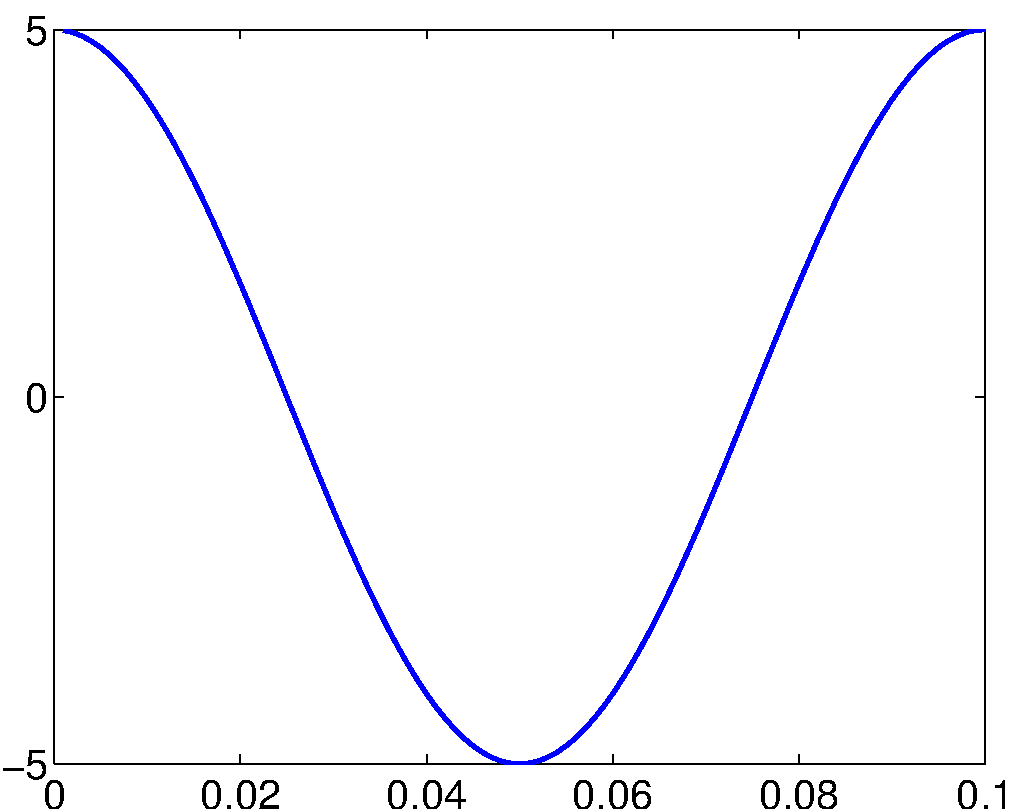
\includegraphics[height=.35\textheight]{sampling_p0.pdf}}
    \subfigure[sampled $x(t)$]{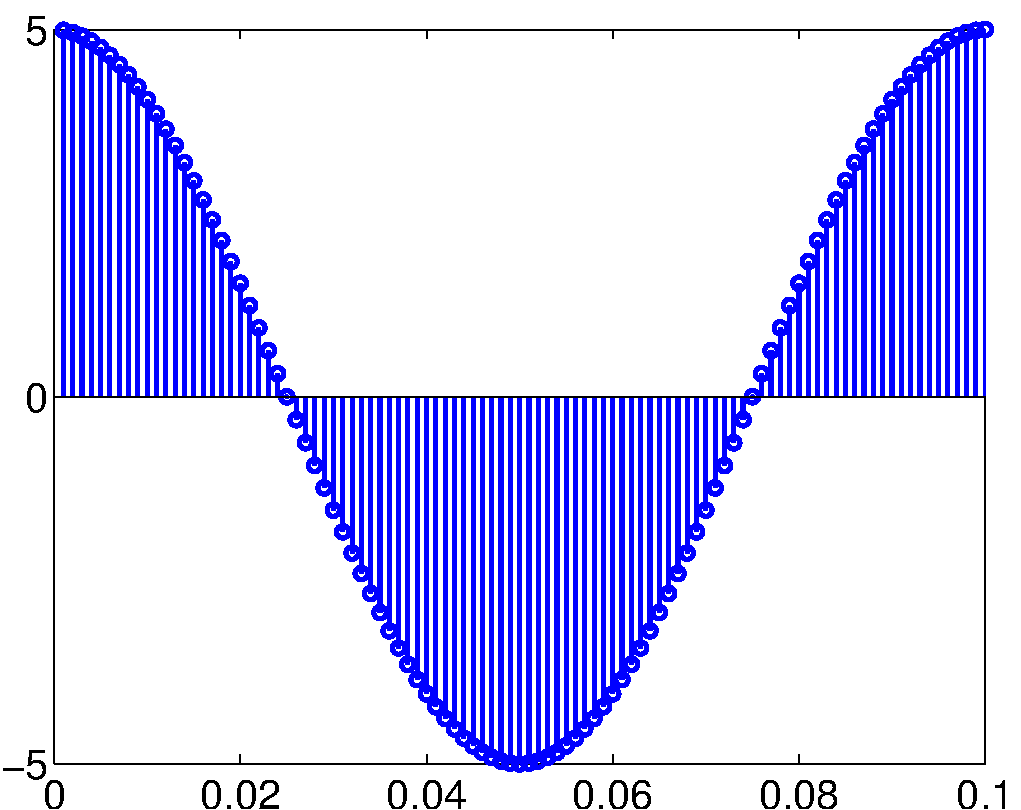
\includegraphics[height=.35\textheight]{sampling_p1.pdf}} \\
    \subfigure[quantized signal]{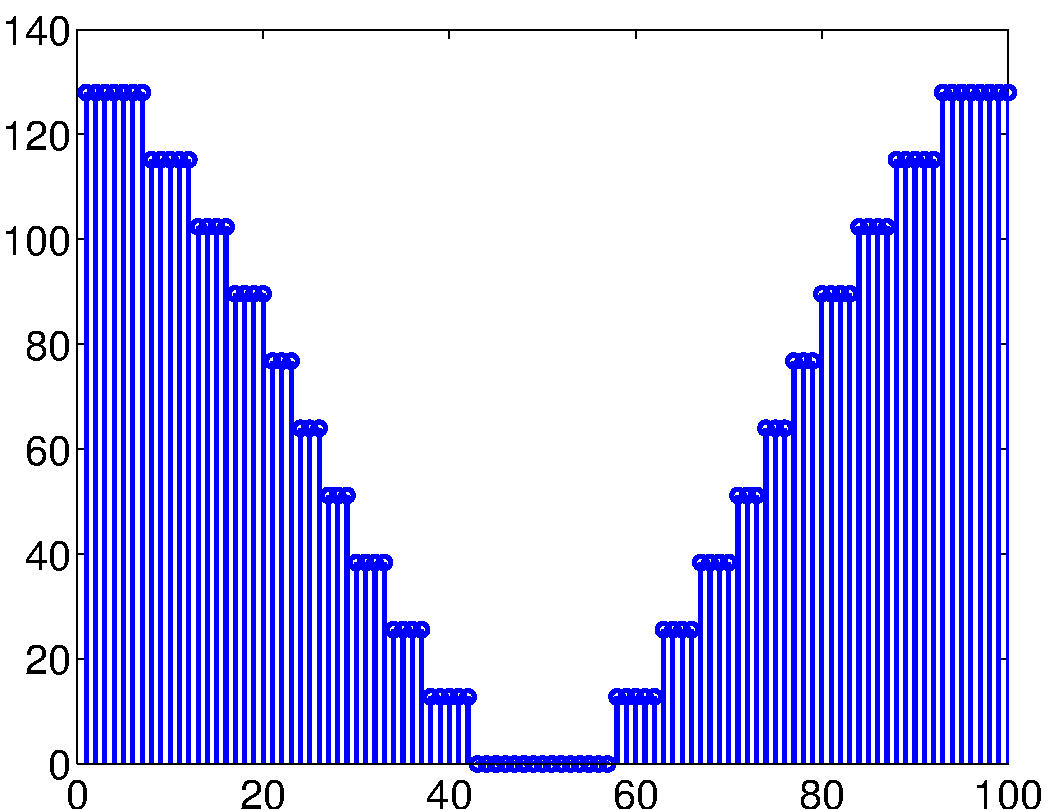
\includegraphics[height=.35\textheight]{sampling_p2.pdf}}
    \subfigure[$\hat{x}(t)$]{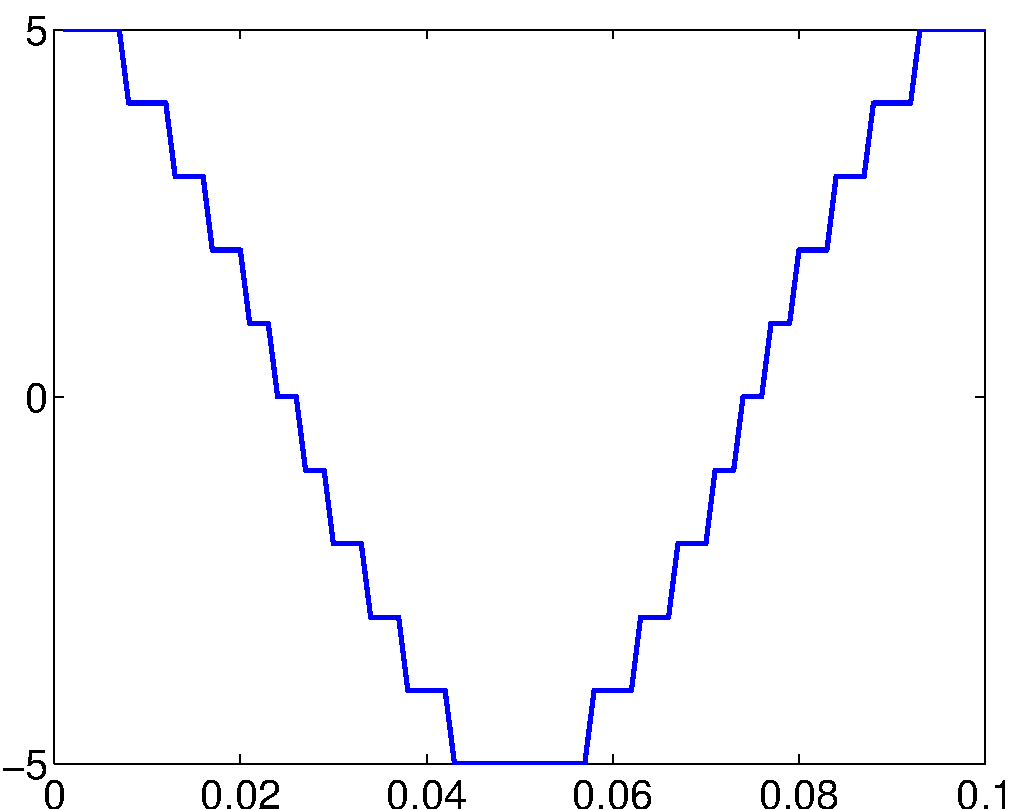
\includegraphics[height=.35\textheight]{sampling_p3.pdf}}  
  \end{figure}
\end{frame}

%--------------------------------------------------------------------------------------------
\begin{frame}\frametitle{Aliasing}\small
  \begin{center}
     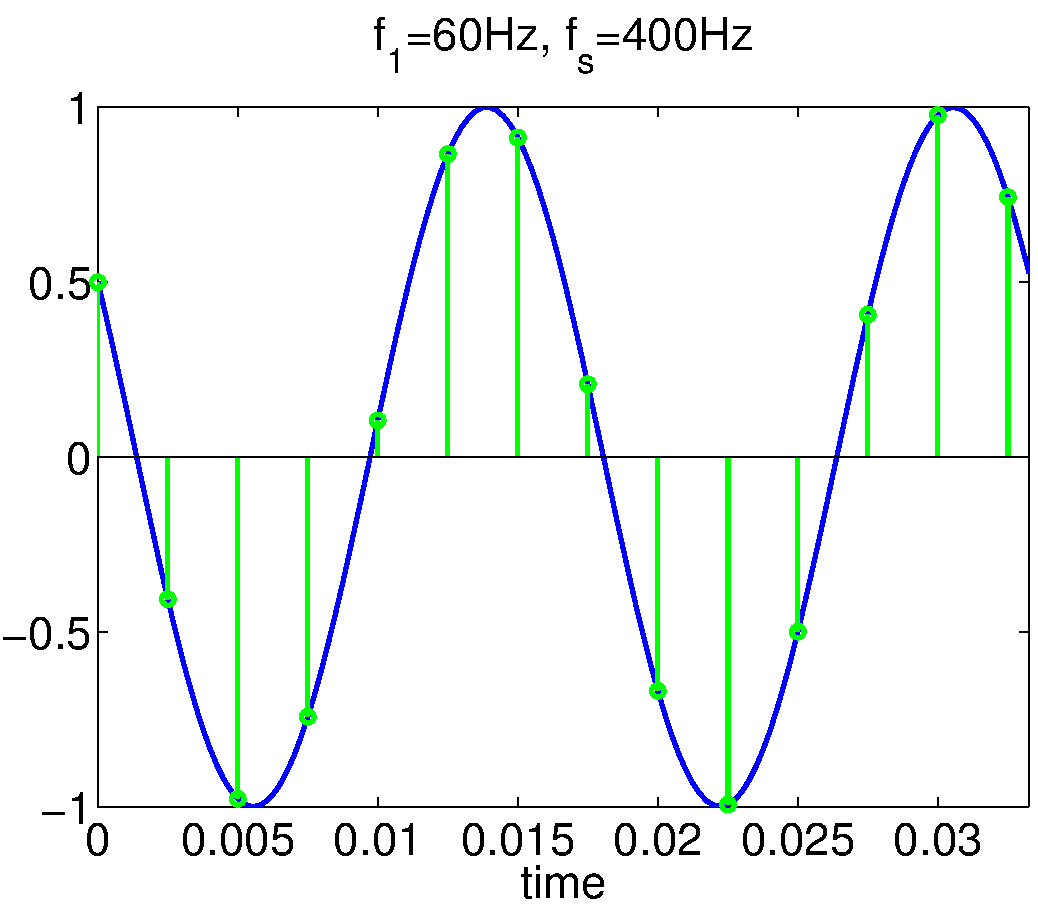
\includegraphics[width=.3\textwidth]{alias01.pdf}\hspace{.2em}
     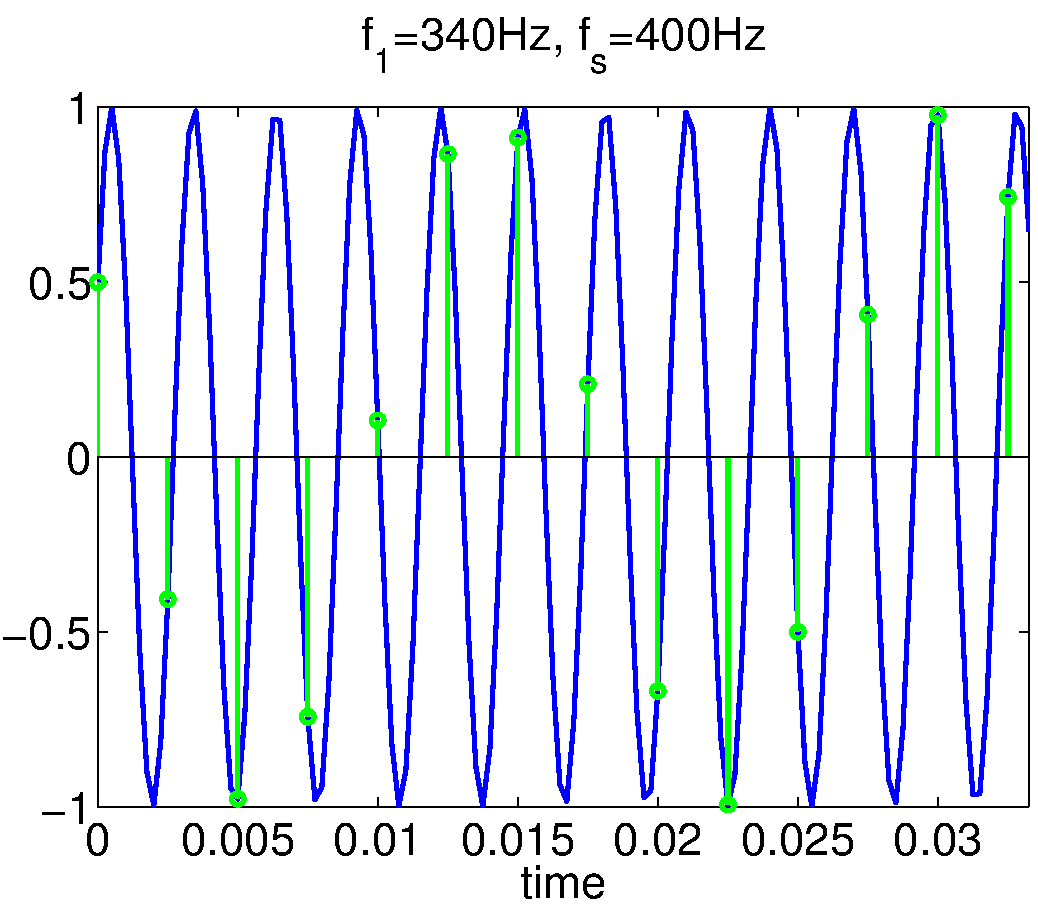
\includegraphics[width=.3\textwidth]{alias02.pdf}\hspace{.2em}
     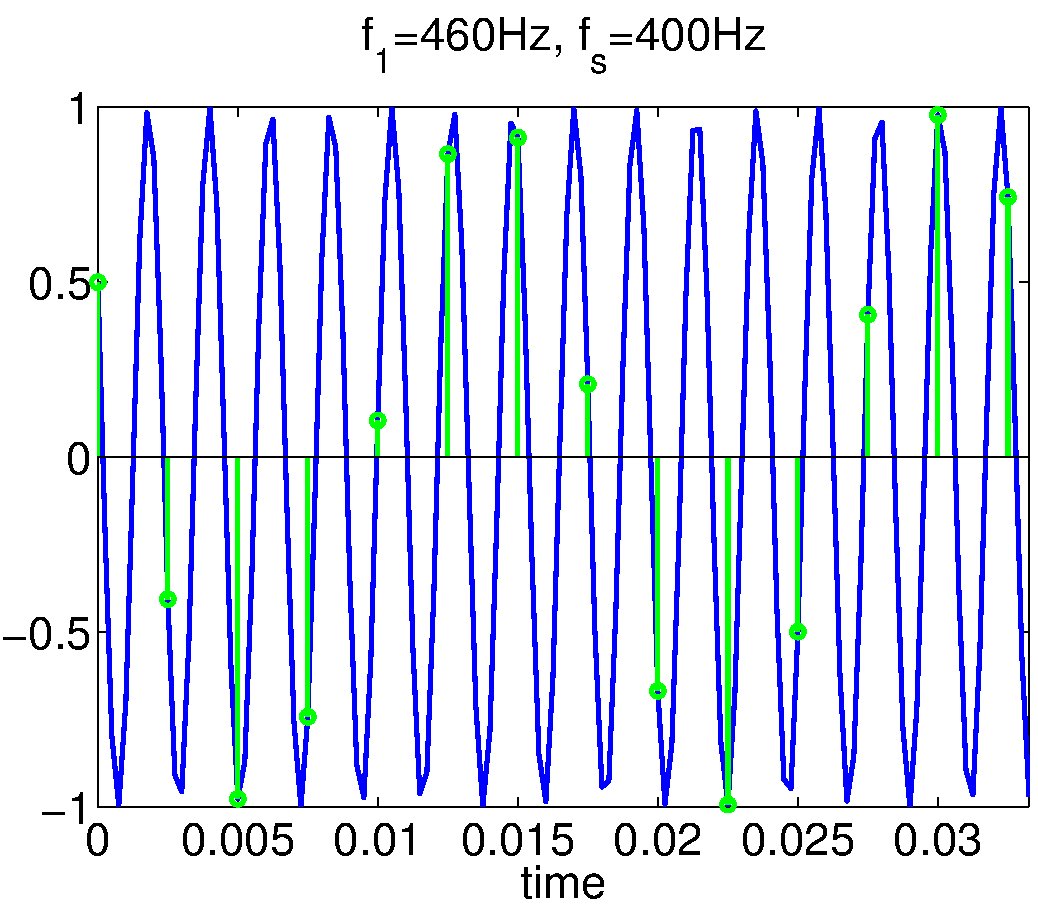
\includegraphics[width=.3\textwidth]{alias03.pdf}
  \end{center}
  \begin{block}{The Sampling Theorem}
    \begin{itemize}
      \item A bandlimited signal can be reconstructed exactly from samples taken with sampling frequency
        \begin{align}
          \frac{1}{T} = f_s \geq  2 f_{\textrm{max}} \nonumber
        \end{align}
    \end{itemize}
  \end{block}
\end{frame}

%--------------------------------------------------------------------------------------------
\begin{frame}\frametitle{Quantization}\small
  \begin{columns}
  \column{.4\textwidth}
    \begin{figure}
    \centering
    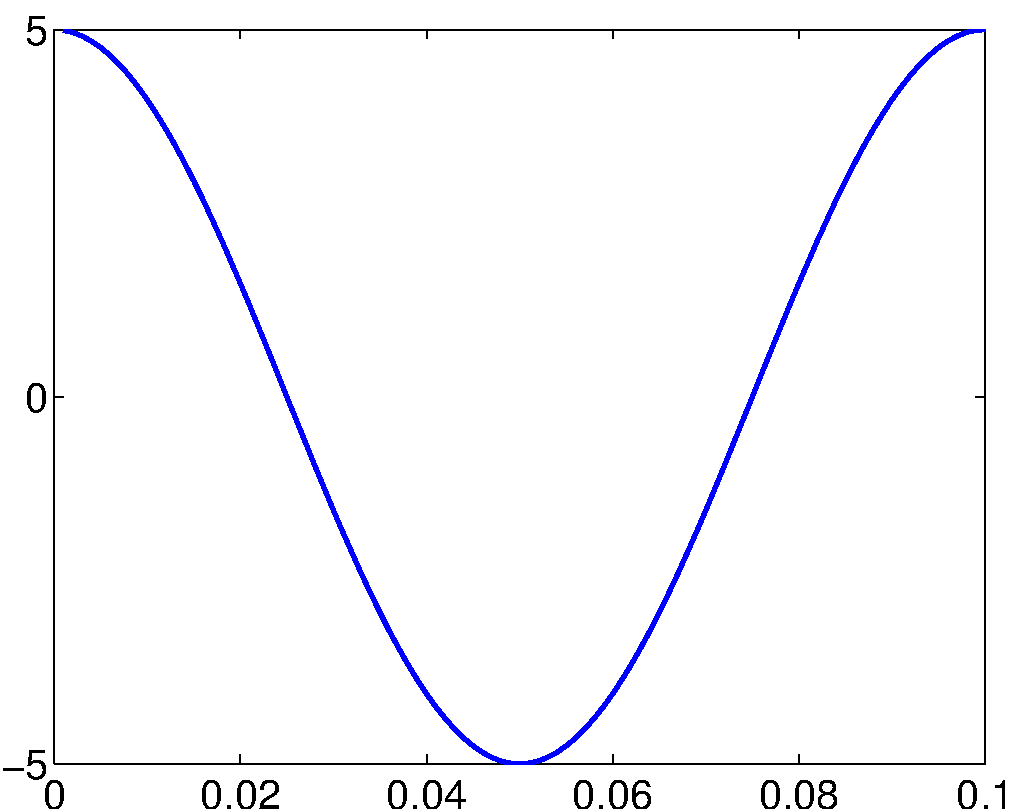
\includegraphics[height=.35\textheight]{sampling_p0.pdf}\\
    $\downarrow$ \\
    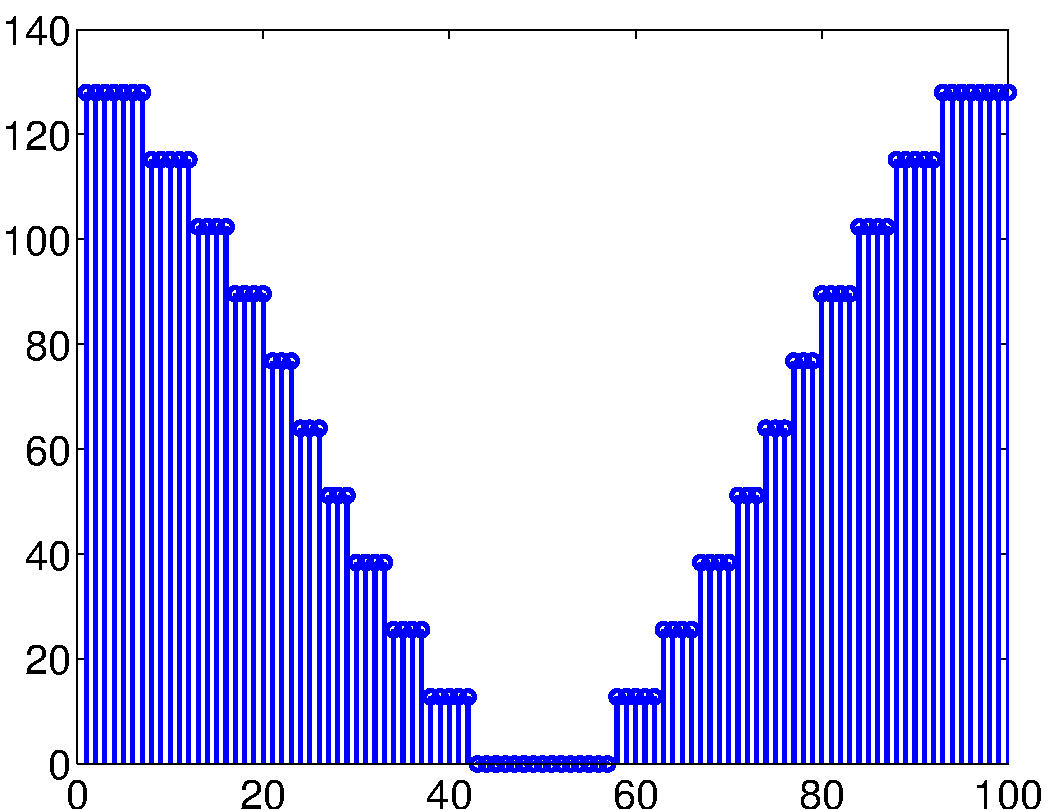
\includegraphics[height=.35\textheight]{sampling_p2.pdf}
    \end{figure}
  \column{.6\textwidth}
    %\includegraphics[width=\textwidth]{Quantization_error.png} \\
    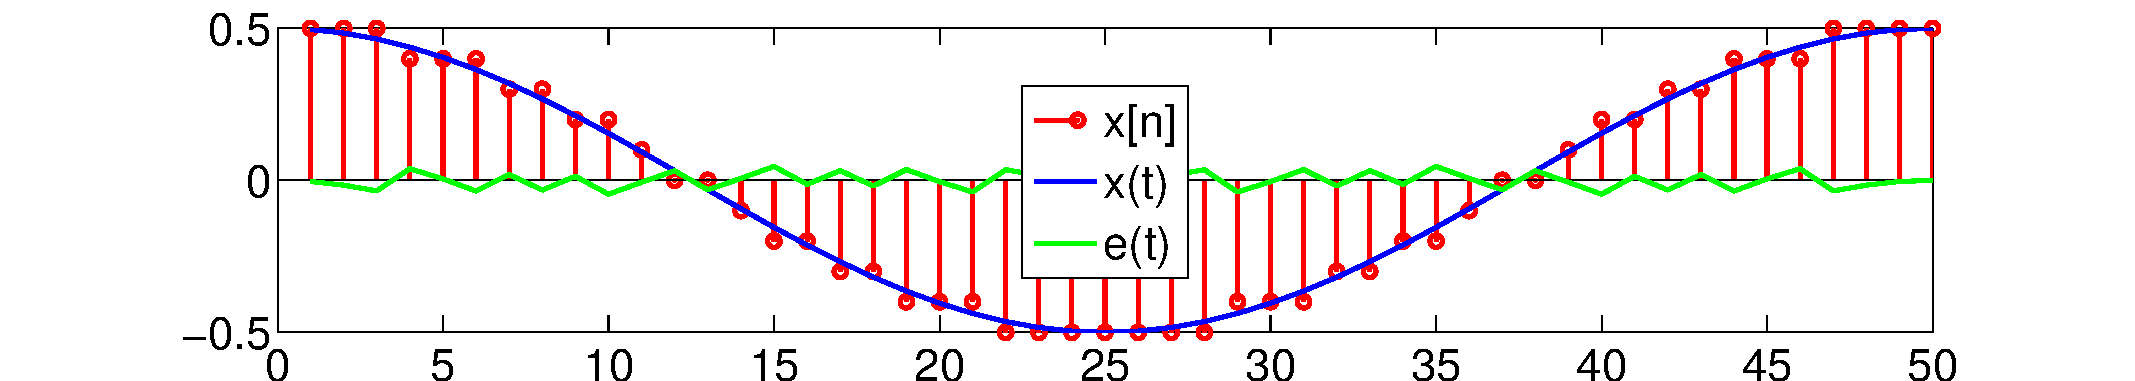
\includegraphics[width=\textwidth]{q_err.pdf} \\
    %{\tiny\url{http://en.wikipedia.org/wiki/Quantization_(signal_processing)}}
    \vspace{1em}
    
    {\color{blue!50!black}\bf Quantization}
    \begin{itemize}
      \item Truncating a continuous signal's discrete representation to a finite set of values. 
        \begin{itemize}
          \item for example, a signal $x(t) \in (\pm 5V)$ is quantized with a resolution of $\frac{10V}{128}$
          \item a form of compression
        \end{itemize} 
      \item Quantization can be  non-uniform for the range of $x(t)$. For example, sampling of voiced speech. 
      \item Quantizing coefficients can have adverse effects to a systems response. Can you think of an example?
    \end{itemize}
  \end{columns}
\end{frame}

%--------------------------------------------------------------------------------------------
\begin{frame}\frametitle{Quantization \& the Elliptic Filter}\small
  %\begin{align}
  %  H(\omega) = \frac{1}{\sqrt{1+\epsilon^2R_n^2(\xi, \omega/\omega_0)}}
  %\end{align}
  \begin{center}
    Pole-Zero plots of an elliptic filter before and after have the coefficients $a_k$ and 
    $b_k$ quantized. \\
    \vspace{1em}
    
    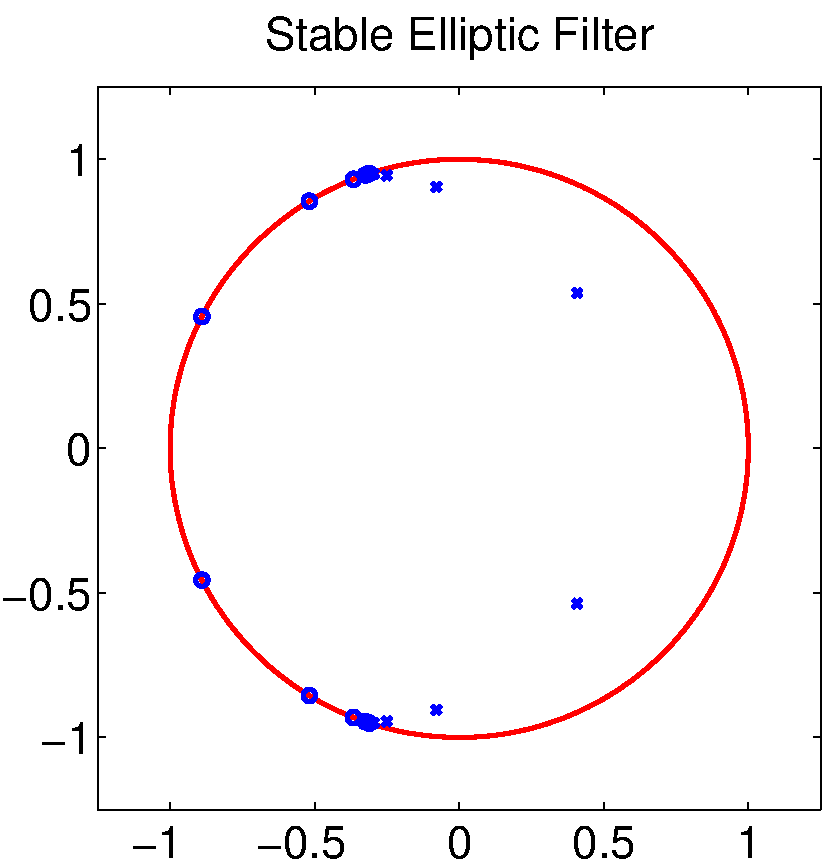
\includegraphics[width=.45\textwidth]{ellip_pz_stable.pdf} \hspace{1em}
    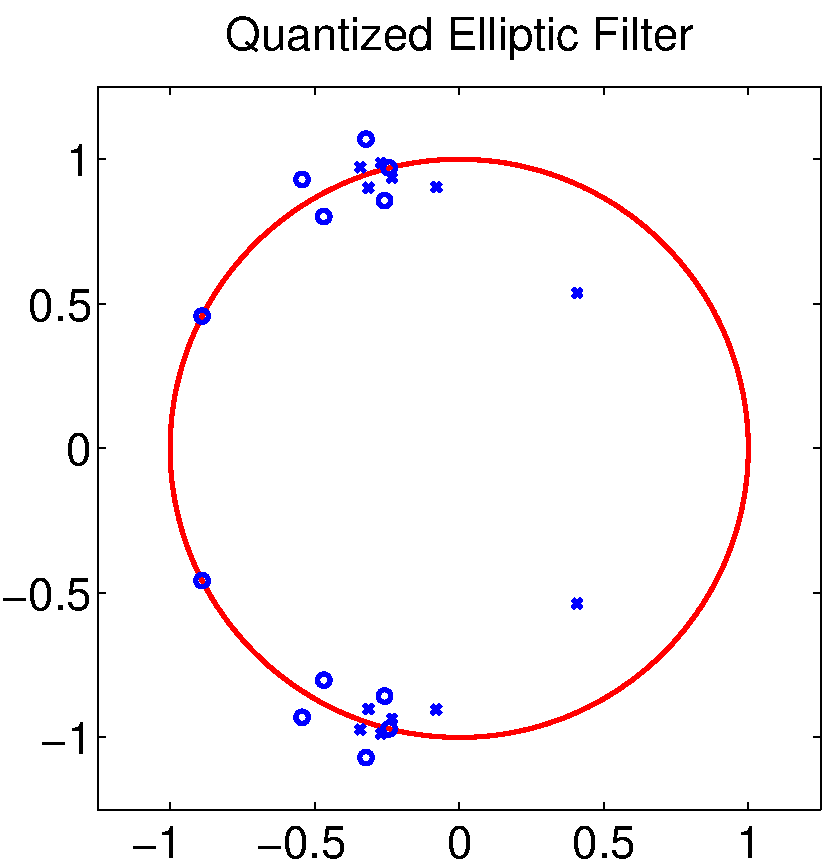
\includegraphics[width=.45\textwidth]{ellip_pz_unstable.pdf}
  \end{center}
\end{frame}


%--------------------------------------------------------------------------------------------
\begin{frame}\frametitle{Quantization \& the Elliptic Filter}\small
  \begin{center}
    Frequency and phase response of an elliptic filter before and after have the coefficients $a_k$ and 
    $b_k$ quantized. \\
    \vspace{1em}
    
    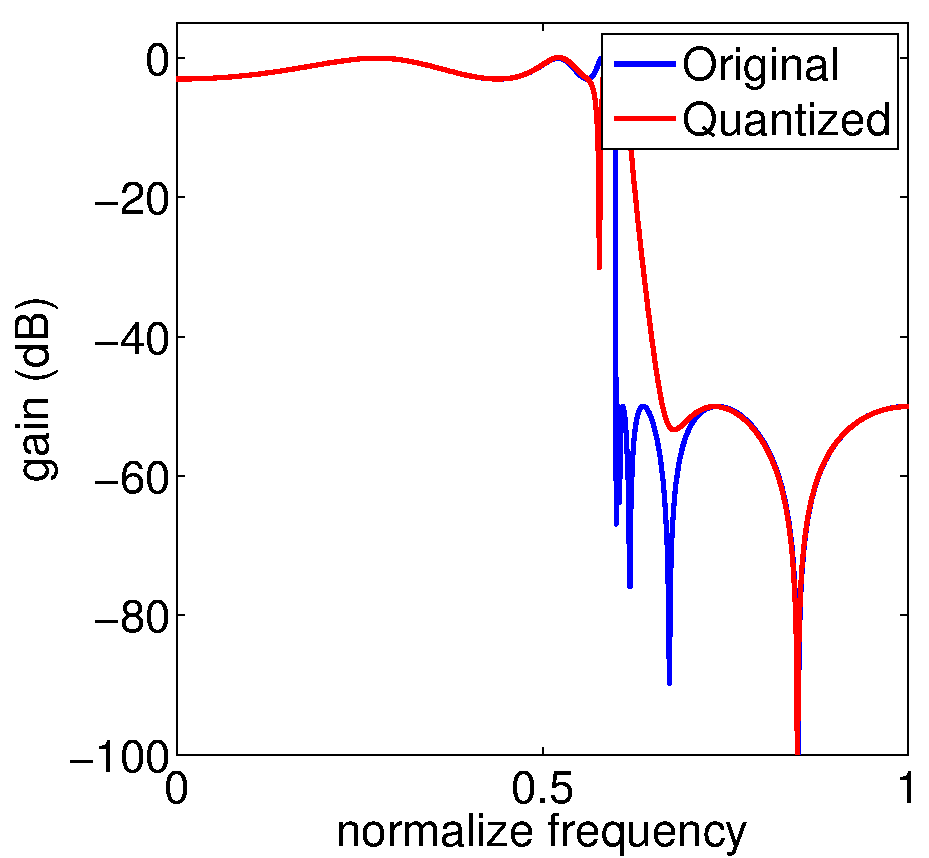
\includegraphics[height=.55\textheight]{ellip_freq.pdf} \hspace{1em}
    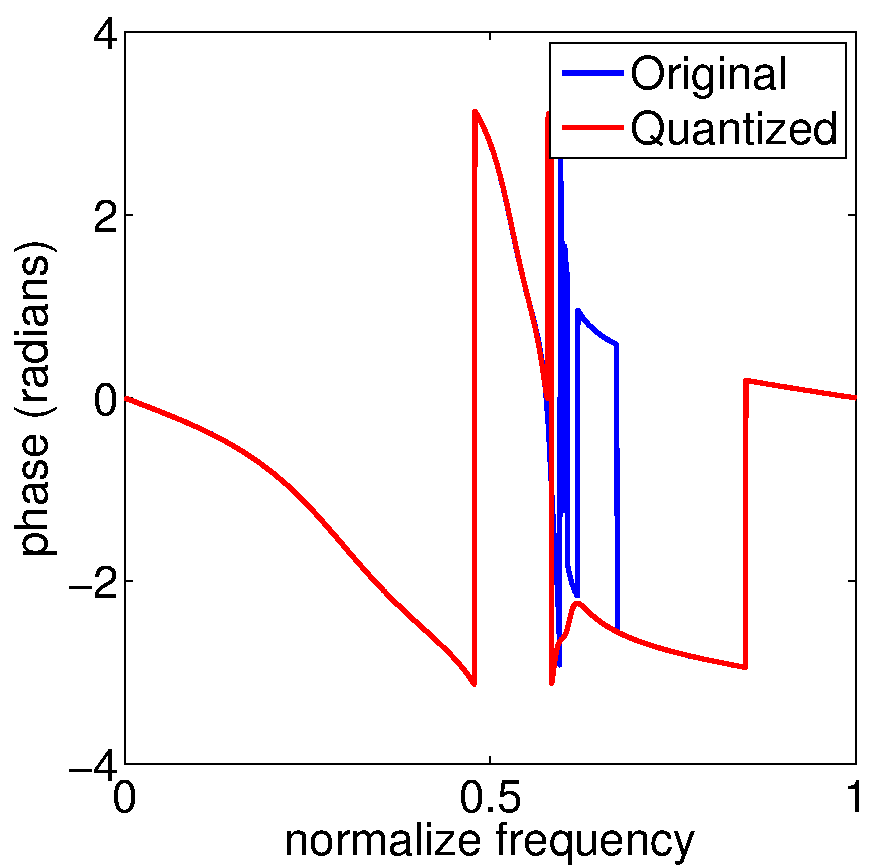
\includegraphics[height=.55\textheight]{ellip_phase.pdf}
  \end{center}
\end{frame}



%--------------------------------------------------------------------------------------------
\begin{frame}\frametitle{Discrete Fourier Transform}\small
  \begin{block}{What's this all about?}
    \begin{itemize}
      \item The Discrete Fourier Transform is a sampled version of the Discrete-Time Fourier Transform with the sampling happening in the frequency domain. We let $\hat{\omega}=\frac{2\pi k}{N}$ then the analysis equation becomes
        \begin{align}
          X[k] = \sum_{n=0}^{N-1} x[n] \e^{-j\frac{2\pi k n}{N}} = \sum_{n=0}^{N-1} x[n] W_N^{kn} \nonumber
        \end{align}
        and the synthesis equation is given by 
        \begin{align}
          x[k] = \sum_{k=0}^{N-1} X[n] \e^{j\frac{2\pi k n}{N}} = \sum_{k=0}^{N-1} X[n] W_N^{-kn} \nonumber
        \end{align}
    \end{itemize}
  \end{block}
\end{frame}


%--------------------------------------------------------------------------------------------
\begin{frame}\frametitle{Clever Manipulations of the Discrete Fourier Transform}\small
  Let us take a moment and begin by decomposing the Discrete Fourier Transform into the sum of the even and odd terms of $n \in [N-1]$.
  \begin{align}
    X[k] &= \sum_{n=0}^{N-1} x[n] \e^{-j\frac{2\pi k n}{N}} = \sum_{n=0}^{(N/2)-1} x[2n] \e^{-j\frac{2\pi k (2n)}{N}} + \sum_{n=0}^{(N/2)-1} x[2n+1] \e^{-j\frac{2\pi k (2n+1)}{N}} \nonumber \\
    &= \sum_{n=0}^{(N/2)-1} x[2n] \e^{-j\frac{2\pi k (2n)}{N}} + \e^{-j\frac{2\pi k}{N}} \sum_{n=0}^{(N/2)-1} x[2n+1] \e^{-j\frac{2\pi k (2n)}{N}}  \nonumber \\
    &= \sum_{n=0}^{(N/2)-1} x[2n] W_N^{2kn} + W_N^{k} \sum_{n=0}^{(N/2)-1} x[2n+1] W_N^{2kn} \nonumber \\
    &= \sum_{n=0}^{(N/2)-1} x[2n] W_{N/2}^{kn} + W_N^{k} \sum_{n=0}^{(N/2)-1} x[2n+1] W_{N/2}^{kn} \nonumber 
  \end{align}
  Let us take a moment to examine the 2nd half of the transform, that is, $\hat{k} = k +N/2$.
\end{frame}


%--------------------------------------------------------------------------------------------
\begin{frame}\frametitle{Clever Manipulations of the Discrete Fourier Transform (cont.)}\small
  Continuing along, 
  \begin{align}
    X[k+N/2] &= \sum_{n=0}^{(N/2)-1} x[2n] W_{N/2}^{(k+N/2)n} + W_N^{k+N/2} \sum_{n=0}^{(N/2)-1} x[2n+1] W_{N/2}^{(k+N/2)n} \nonumber 
  \end{align}
  After some examination, we see that $W_{N/2}^{(k+N/2)n} = W_{N/2}^{kn} W_{N/2}^{nN/2} = W_{N/2}^{kn} \e^{-j2\pi n 2N/(2N)} = W_{N/2}^{kn}$. Also, $W_N^{k+N/2} =  -W_N^{k}$. Then 
  \begin{align}
    X[k+N/2] &= \sum_{n=0}^{(N/2)-1} x[2n] W_{N/2}^{kn} -W_N^{k} \sum_{n=0}^{(N/2)-1} x[2n+1] W_{N/2}^{kn}\nonumber 
  \end{align}
  and recall that 
  \begin{align}
    X[k] &= \sum_{n=0}^{(N/2)-1} x[2n] W_{N/2}^{kn} + W_N^{k} \sum_{n=0}^{(N/2)-1} x[2n+1] W_{N/2}^{kn} \nonumber 
  \end{align}
  Okay\ldots What did we just show? 
\end{frame}


%--------------------------------------------------------------------------------------------
\begin{frame}\frametitle{Ladies \& Gentlemen: I give you the Fast Fourier Transform}\small
  \begin{block}{Decimation in Time FFT}
    \begin{itemize}
      \item We derived the basis for a radix-2 decimation in time FFT algorithm. The terms $W_N^{k}$ are called ``twiddle'' factors and we assume $N$ is a power of 2. 
    \end{itemize}
  \end{block}
\end{frame}


%--------------------------------------------------------------------------------------------
\begin{frame}\frametitle{FFT in one picture}\small
  \begin{center}
    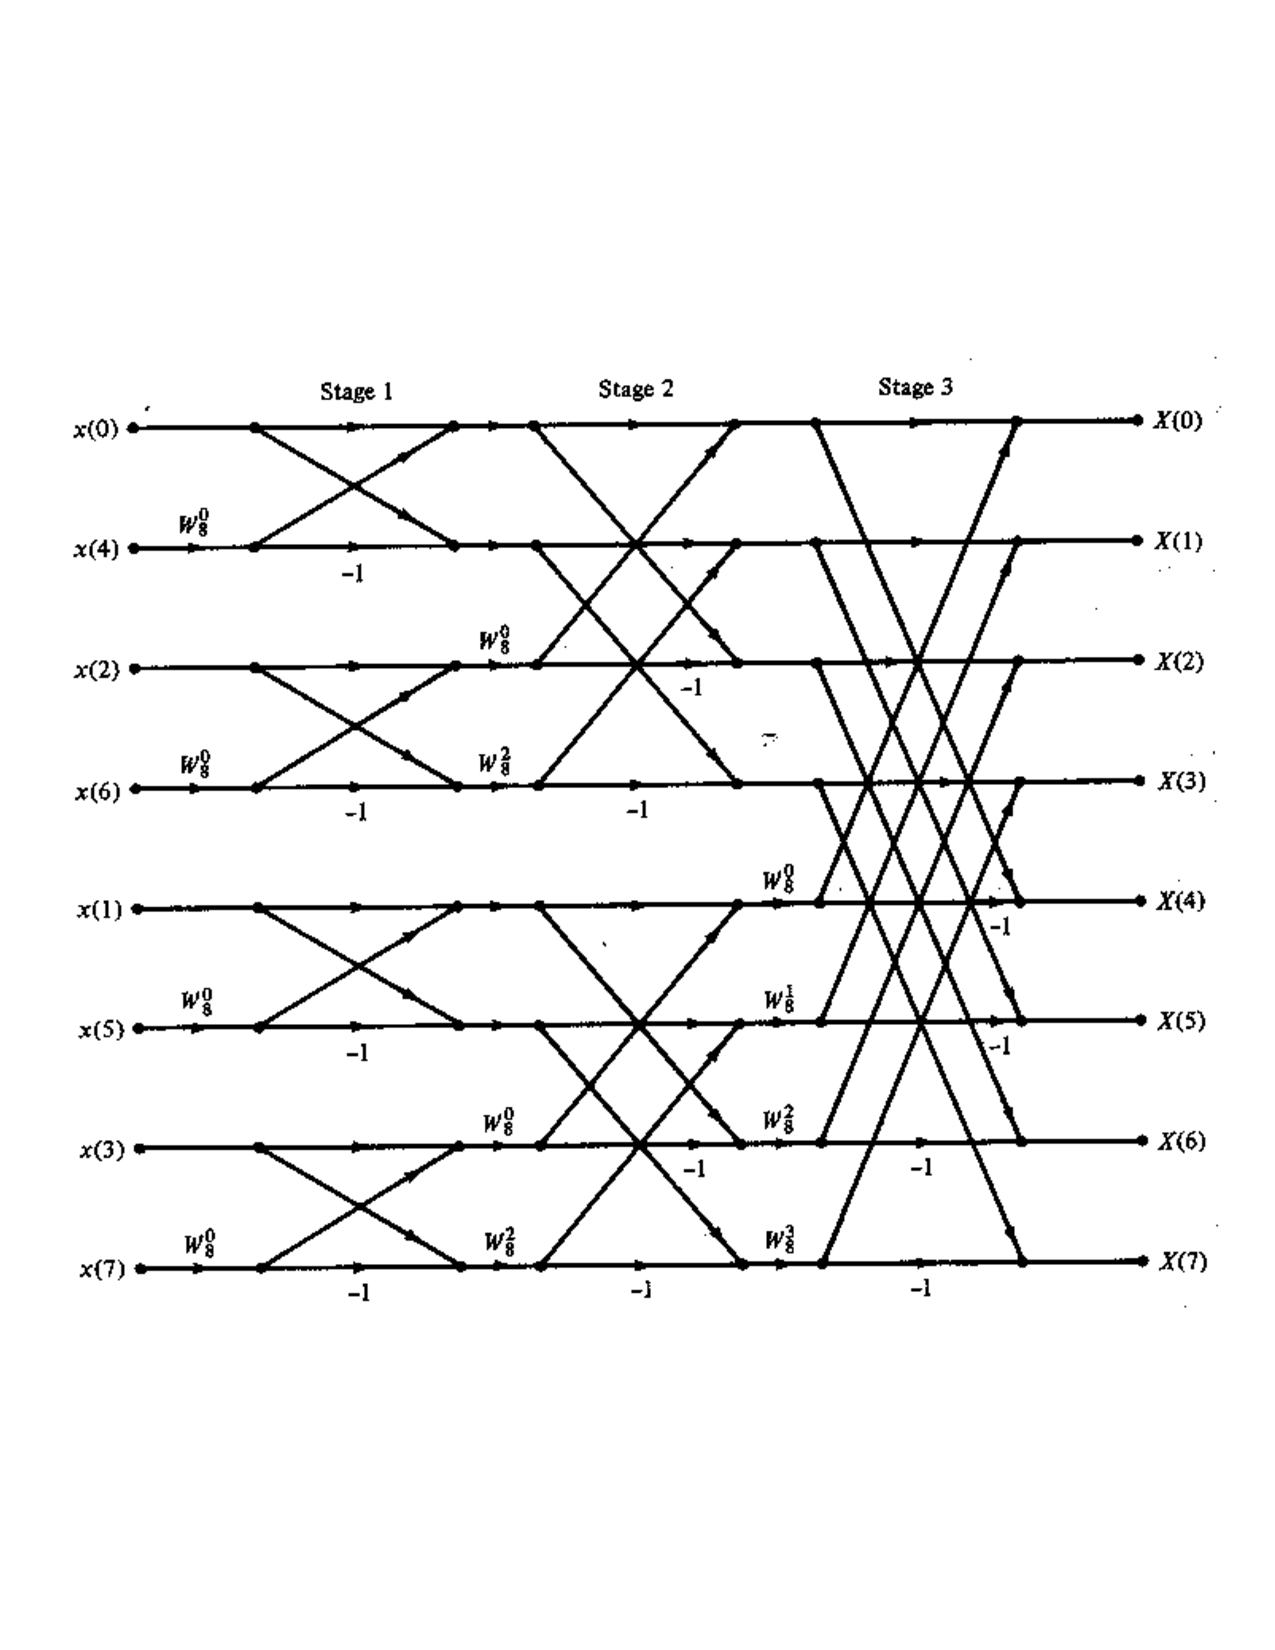
\includegraphics[height=\textheight]{fft.pdf}
  \end{center}
\end{frame}


%--------------------------------------------------------------------------------------------
\begin{frame}\frametitle{$Z$-transform}\small
  \begin{block}{What is the $Z$-transform: In words}
    \begin{itemize}
      \item The $Z$-transform is a little more general than the discrete-time Fourier transform. In fact, the discrete-time Fourier transform is a special can case of the $Z$-transform. The DTFT is the $Z$-transform being evaluated on the unit circle. 
      \item The $Z$-transform of a sequence $x[n]$ must have its region of convergence within the unit circle for the DTFT to exist. 
      \item The $Z$-transform is the discrete cousin of the Laplace transform. 
    \end{itemize}
  \end{block}
  
  \begin{exampleblock}{What is the $Z$-transform: In equations}
    \begin{itemize}
      \item The $Z$-transform is defined by
        \begin{align}
          X(z) = \sum_{n=-\infty}^{\infty} x[n] z^{-n} 
          \nonumber
        \end{align}
        where $z \in \mathbb{C}$.
      \item The set of values for $z$ where the Laurent series converges is called the {\em\color{green!50!black}region of convergence}. 
        \begin{align}
          \sum_{n=-\infty}^{\infty} |x[n]| |z|^{-n} \leq \infty
          \nonumber
        \end{align}
    \end{itemize}
  \end{exampleblock}
\end{frame}


%--------------------------------------------------------------------------------------------
\begin{frame}\frametitle{$Z$-transform}\small
  \begin{block}{$Z$-transform}
    \begin{itemize}
      \item The $Z$-transform can {\em\color{blue!50!black}generally} be written as a ratio of polynomials of $z$.
        \begin{align}
          X(z) =\frac{P(z)}{Q(z)}
          \nonumber
        \end{align} 
        The roots of $P(z)$ and $Q(z)$ are called the {\em\color{blue!50!black}zeros} and {\em\color{blue!50!black}poles}, respectively. 
      \item Poles could occur at $z=0$ or $|z|=\infty$. The locations of the poles are very important for determining the region of convergence. 
    \end{itemize}
  \end{block}
\end{frame}

%--------------------------------------------------------------------------------------------
\begin{frame}\frametitle{$Z$-transform (Example)}\small
  Consider the signal $x[n] = a^n u[n]$. Because it is non-zero for only $n \geq 0$, this is an example of a right-sided sequence. By definition, 
  \begin{align}
    X(z) = \sum_{n=-\infty}^{\infty} a^n u[n] z^{-n} = \sum_{n=0}^{\infty} (az^{-1})^n \nonumber
  \end{align}
  For convergence of $X(z)$, we need
  \begin{align}
     \sum_{n=0}^{\infty} |az^{-1}|^n  \leq \infty\nonumber
  \end{align}
  Thus the ROC is all the values for $z$ where $|az^{-1}| < 1$ or $|a| < |z|$.  Then 
  \begin{align}
    X(z)  = \sum_{n=0}^{\infty} (az^{-1})^n  = \frac{1}{1 - az^{-1}} = \frac{z}{z-a} \nonumber
  \end{align}
  only if $|a| < |z|$.
\end{frame}



%--------------------------------------------------------------------------------------------
\begin{frame}\frametitle{$Z$-transform (Example)}\small

  \begin{columns}
    \column{.5\textwidth}
      \begin{block}{Question}
      Given the system
      \begin{align}
        H(z) = \e^{z^{-1}} \nonumber
      \end{align}
      What is $h[n]$? What is the ROC? Is the system BIBO stable?
      \end{block}
    \column{.5\textwidth} \footnotesize
      \uncover<2->{
      {\bf\color{blue!50!black}Solution}\\
      Directly apply the Lorentz series expansion to $H(z)$
      \begin{align}
        H(z) &= \e^{z^{-1}} = 1 + z^{-1} + \frac{1}{2!}z^{-2} +\cdots \nonumber \\
        &= \sum_{n=0}^{\infty} h[n] u[n]\nonumber
      \end{align}
      Thus, $h[n] = \frac{1}{n!}u[n]$. Is the system BIBO stable?} \uncover<3->{Apply the ratio test to see if the series converges, diverges, or neither.
      \begin{align}
        \lim_{n\rightarrow\infty} \frac{h[n+1]}{h[n]} &= \lim_{n\rightarrow\infty} \frac{n!}{(n+1)!} = \lim_{n\rightarrow\infty} \frac{n!}{(n+1)n!}\nonumber \\
        &= \lim_{n\rightarrow\infty} \frac{1}{n+1} = 0\nonumber
      \end{align}
      Therefore, $H(z)$ is BIBO stable. } \uncover<4->{Examining $H(z)$, we see there are no poles or zeros. Only an essential singularity. ROC is all $z$ except @ 0.}
  \end{columns}
\end{frame}







\end{document}
